\documentclass[1p]{elsarticle_modified}
%\bibliographystyle{elsarticle-num}

%\usepackage[colorlinks]{hyperref}
%\usepackage{abbrmath_seonhwa} %\Abb, \Ascr, \Acal ,\Abf, \Afrak
\usepackage{amsfonts}
\usepackage{amssymb}
\usepackage{amsmath}
\usepackage{amsthm}
\usepackage{scalefnt}
\usepackage{amsbsy}
\usepackage{kotex}
\usepackage{caption}
\usepackage{subfig}
\usepackage{color}
\usepackage{graphicx}
\usepackage{xcolor} %% white, black, red, green, blue, cyan, magenta, yellow
\usepackage{float}
\usepackage{setspace}
\usepackage{hyperref}

\usepackage{tikz}
\usetikzlibrary{arrows}

\usepackage{multirow}
\usepackage{array} % fixed length table
\usepackage{hhline}

%%%%%%%%%%%%%%%%%%%%%
\makeatletter
\renewcommand*\env@matrix[1][\arraystretch]{%
	\edef\arraystretch{#1}%
	\hskip -\arraycolsep
	\let\@ifnextchar\new@ifnextchar
	\array{*\c@MaxMatrixCols c}}
\makeatother %https://tex.stackexchange.com/questions/14071/how-can-i-increase-the-line-spacing-in-a-matrix
%%%%%%%%%%%%%%%

\usepackage[normalem]{ulem}

\newcommand{\msout}[1]{\ifmmode\text{\sout{\ensuremath{#1}}}\else\sout{#1}\fi}
%SOURCE: \msout is \stkout macro in https://tex.stackexchange.com/questions/20609/strikeout-in-math-mode

\newcommand{\cancel}[1]{
	\ifmmode
	{\color{red}\msout{#1}}
	\else
	{\color{red}\sout{#1}}
	\fi
}

\newcommand{\add}[1]{
	{\color{blue}\uwave{#1}}
}

\newcommand{\replace}[2]{
	\ifmmode
	{\color{red}\msout{#1}}{\color{blue}\uwave{#2}}
	\else
	{\color{red}\sout{#1}}{\color{blue}\uwave{#2}}
	\fi
}

\newcommand{\Sol}{\mathcal{S}} %segment
\newcommand{\D}{D} %diagram
\newcommand{\A}{\mathcal{A}} %arc


%%%%%%%%%%%%%%%%%%%%%%%%%%%%%5 test

\def\sl{\operatorname{\textup{SL}}(2,\Cbb)}
\def\psl{\operatorname{\textup{PSL}}(2,\Cbb)}
\def\quan{\mkern 1mu \triangleright \mkern 1mu}

\theoremstyle{definition}
\newtheorem{thm}{Theorem}[section]
\newtheorem{prop}[thm]{Proposition}
\newtheorem{lem}[thm]{Lemma}
\newtheorem{ques}[thm]{Question}
\newtheorem{cor}[thm]{Corollary}
\newtheorem{defn}[thm]{Definition}
\newtheorem{exam}[thm]{Example}
\newtheorem{rmk}[thm]{Remark}
\newtheorem{alg}[thm]{Algorithm}

\newcommand{\I}{\sqrt{-1}}
\begin{document}

%\begin{frontmatter}
%
%\title{Boundary parabolic representations of knots up to 8 crossings}
%
%%% Group authors per affiliation:
%\author{Yunhi Cho} 
%\address{Department of Mathematics, University of Seoul, Seoul, Korea}
%\ead{yhcho@uos.ac.kr}
%
%
%\author{Seonhwa Kim} %\fnref{s_kim}}
%\address{Center for Geometry and Physics, Institute for Basic Science, Pohang, 37673, Korea}
%\ead{ryeona17@ibs.re.kr}
%
%\author{Hyuk Kim}
%\address{Department of Mathematical Sciences, Seoul National University, Seoul 08826, Korea}
%\ead{hyukkim@snu.ac.kr}
%
%\author{Seokbeom Yoon}
%\address{Department of Mathematical Sciences, Seoul National University, Seoul, 08826,  Korea}
%\ead{sbyoon15@snu.ac.kr}
%
%\begin{abstract}
%We find all boundary parabolic representation of knots up to 8 crossings.
%
%\end{abstract}
%\begin{keyword}
%    \MSC[2010] 57M25 
%\end{keyword}
%
%\end{frontmatter}

%\linenumbers
%\tableofcontents
%
\newcommand\colored[1]{\textcolor{white}{\rule[-0.35ex]{0.8em}{1.4ex}}\kern-0.8em\color{red} #1}%
%\newcommand\colored[1]{\textcolor{white}{ #1}\kern-2.17ex	\textcolor{white}{ #1}\kern-1.81ex	\textcolor{white}{ #1}\kern-2.15ex\color{red}#1	}

{\Large $\underline{12n_{0518}~(K12n_{0518})}$}

\setlength{\tabcolsep}{10pt}
\renewcommand{\arraystretch}{1.6}
\vspace{1cm}\begin{tabular}{m{100pt}>{\centering\arraybackslash}m{274pt}}
\multirow{5}{120pt}{
	\centering
	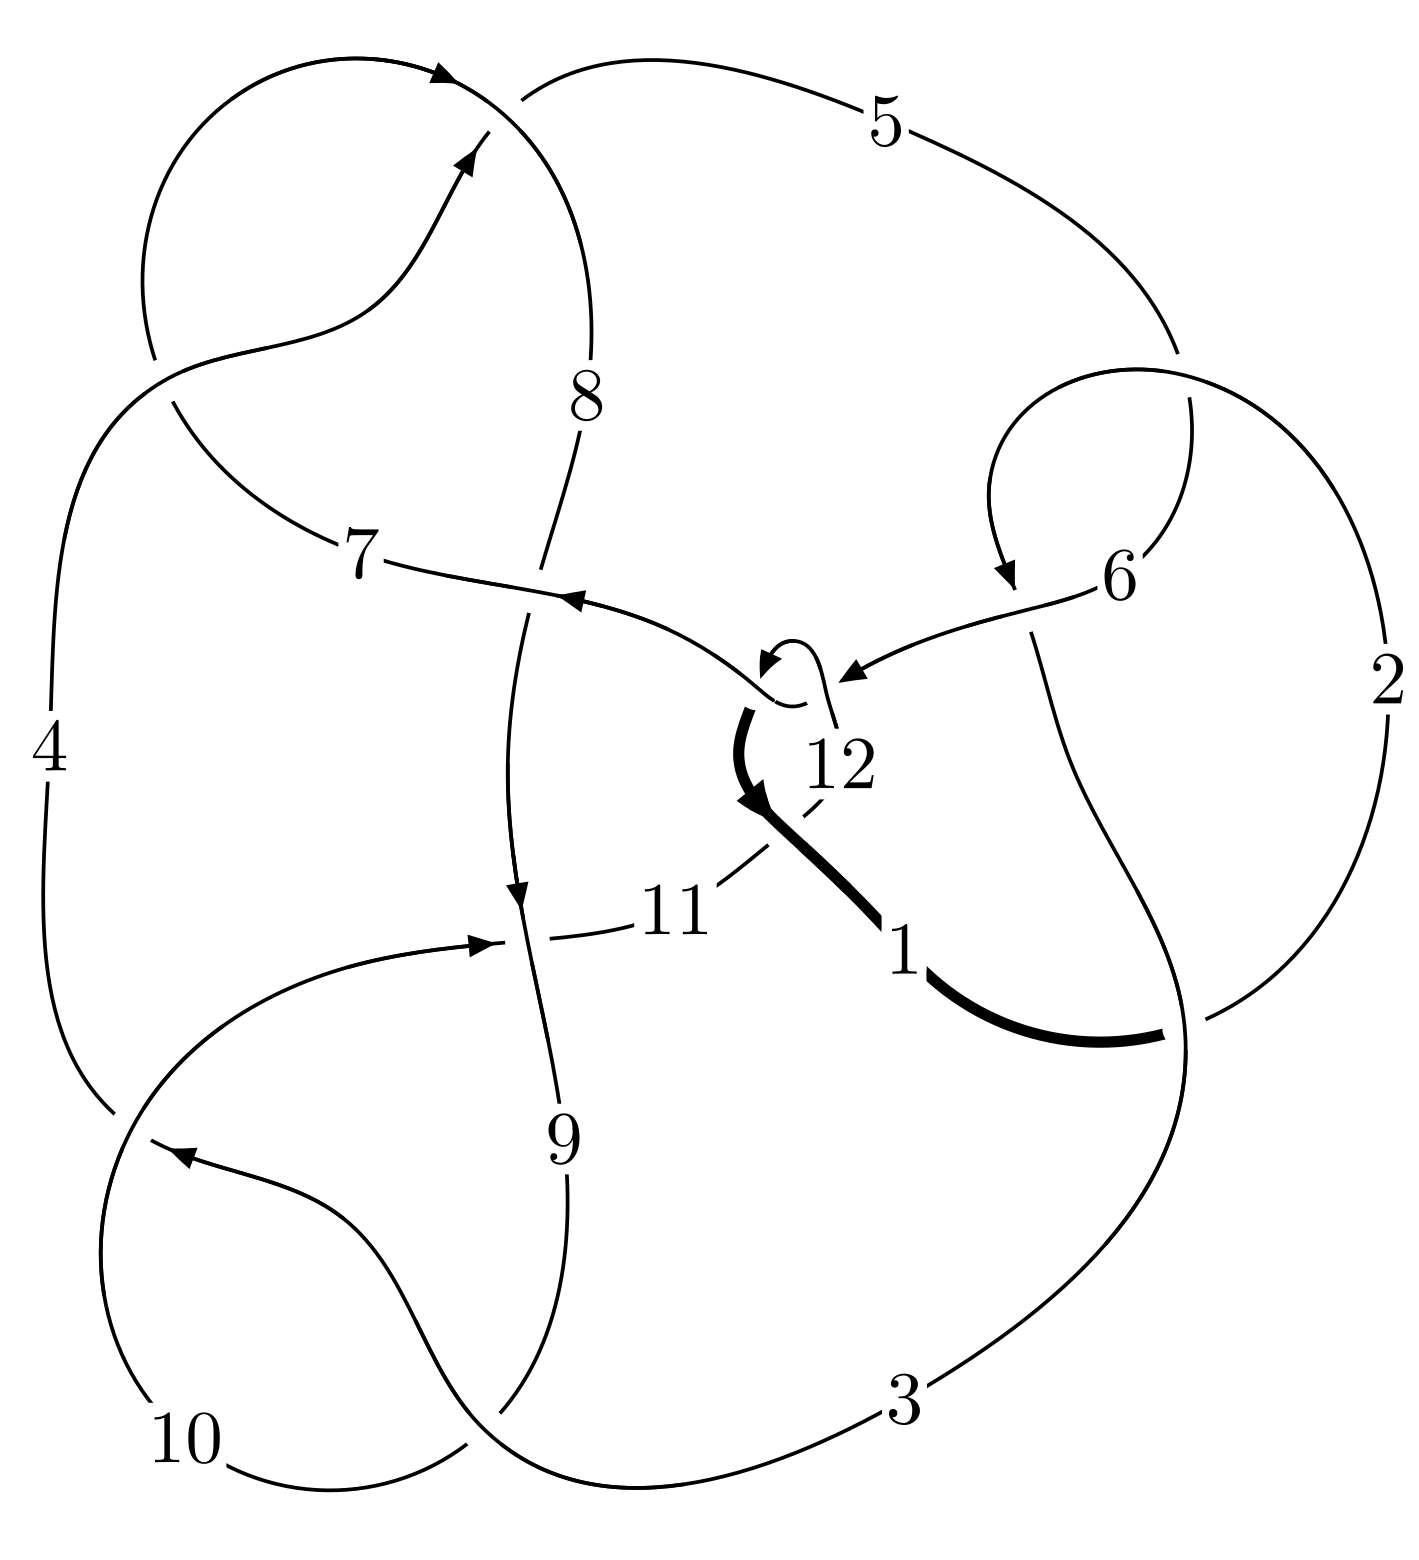
\includegraphics[width=112pt]{../../../GIT/diagram.site/Diagrams/png/2607_12n_0518.png}\\
\ \ \ A knot diagram\footnotemark}&
\allowdisplaybreaks
\textbf{Linearized knot diagam} \\
\cline{2-2}
 &
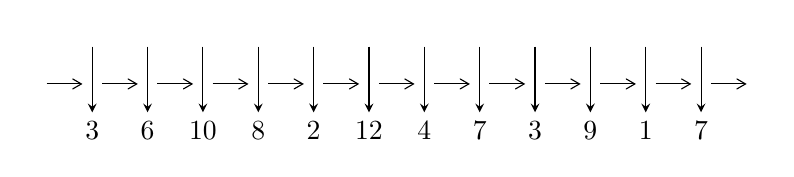
\begin{tikzpicture}[x=20pt, y=17pt]
	% nodes
	\node (C0) at (0, 0) {};
	\node (C1) at (1, 0) {};
	\node (C1U) at (1, +1) {};
	\node (C1D) at (1, -1) {3};

	\node (C2) at (2, 0) {};
	\node (C2U) at (2, +1) {};
	\node (C2D) at (2, -1) {6};

	\node (C3) at (3, 0) {};
	\node (C3U) at (3, +1) {};
	\node (C3D) at (3, -1) {10};

	\node (C4) at (4, 0) {};
	\node (C4U) at (4, +1) {};
	\node (C4D) at (4, -1) {8};

	\node (C5) at (5, 0) {};
	\node (C5U) at (5, +1) {};
	\node (C5D) at (5, -1) {2};

	\node (C6) at (6, 0) {};
	\node (C6U) at (6, +1) {};
	\node (C6D) at (6, -1) {12};

	\node (C7) at (7, 0) {};
	\node (C7U) at (7, +1) {};
	\node (C7D) at (7, -1) {4};

	\node (C8) at (8, 0) {};
	\node (C8U) at (8, +1) {};
	\node (C8D) at (8, -1) {7};

	\node (C9) at (9, 0) {};
	\node (C9U) at (9, +1) {};
	\node (C9D) at (9, -1) {3};

	\node (C10) at (10, 0) {};
	\node (C10U) at (10, +1) {};
	\node (C10D) at (10, -1) {9};

	\node (C11) at (11, 0) {};
	\node (C11U) at (11, +1) {};
	\node (C11D) at (11, -1) {1};

	\node (C12) at (12, 0) {};
	\node (C12U) at (12, +1) {};
	\node (C12D) at (12, -1) {7};
	\node (C13) at (13, 0) {};

	% arrows
	\draw[->,>={angle 60}]
	(C0) edge (C1) (C1) edge (C2) (C2) edge (C3) (C3) edge (C4) (C4) edge (C5) (C5) edge (C6) (C6) edge (C7) (C7) edge (C8) (C8) edge (C9) (C9) edge (C10) (C10) edge (C11) (C11) edge (C12) (C12) edge (C13) ;	\draw[->,>=stealth]
	(C1U) edge (C1D) (C2U) edge (C2D) (C3U) edge (C3D) (C4U) edge (C4D) (C5U) edge (C5D) (C6U) edge (C6D) (C7U) edge (C7D) (C8U) edge (C8D) (C9U) edge (C9D) (C10U) edge (C10D) (C11U) edge (C11D) (C12U) edge (C12D) ;
	\end{tikzpicture} \\
\hhline{~~} \\& 
\textbf{Solving Sequence} \\ \cline{2-2} 
 &
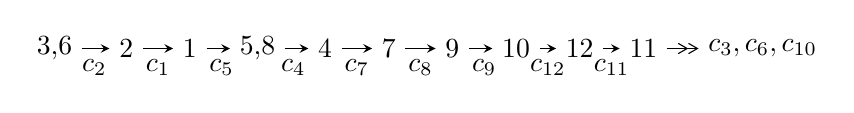
\begin{tikzpicture}[x=23pt, y=7pt]
	% node
	\node (A0) at (-1/8, 0) {3,6};
	\node (A1) at (1, 0) {2};
	\node (A2) at (2, 0) {1};
	\node (A3) at (49/16, 0) {5,8};
	\node (A4) at (33/8, 0) {4};
	\node (A5) at (41/8, 0) {7};
	\node (A6) at (49/8, 0) {9};
	\node (A7) at (57/8, 0) {10};
	\node (A8) at (65/8, 0) {12};
	\node (A9) at (73/8, 0) {11};
	\node (C1) at (1/2, -1) {$c_{2}$};
	\node (C2) at (3/2, -1) {$c_{1}$};
	\node (C3) at (5/2, -1) {$c_{5}$};
	\node (C4) at (29/8, -1) {$c_{4}$};
	\node (C5) at (37/8, -1) {$c_{7}$};
	\node (C6) at (45/8, -1) {$c_{8}$};
	\node (C7) at (53/8, -1) {$c_{9}$};
	\node (C8) at (61/8, -1) {$c_{12}$};
	\node (C9) at (69/8, -1) {$c_{11}$};
	\node (A10) at (11, 0) {$c_{3},c_{6},c_{10}$};

	% edge
	\draw[->,>=stealth]	
	(A0) edge (A1) (A1) edge (A2) (A2) edge (A3) (A3) edge (A4) (A4) edge (A5) (A5) edge (A6) (A6) edge (A7) (A7) edge (A8) (A8) edge (A9) ;
	\draw[->>,>={angle 60}]	
	(A9) edge (A10);
\end{tikzpicture} \\ 

\end{tabular} \\

\footnotetext{
The image of knot diagram is generated by the software ``\textbf{Draw programme}" developed by Andrew Bartholomew(\url{http://www.layer8.co.uk/maths/draw/index.htm\#Running-draw}), where we modified some parts for our purpose(\url{https://github.com/CATsTAILs/LinksPainter}).
}\phantom \\ \newline 
\centering \textbf{Ideals for irreducible components\footnotemark of $X_{\text{par}}$} 
 
\begin{align*}
I^u_{1}&=\langle 
u^2+b+u-1,\;u^4- u^2+2 a+u+1,\;u^5- u^4- u^3+2 u^2+2 u-1\rangle \\
I^u_{2}&=\langle 
u^6 a+u^5 a+u^6+u^4 a+u^5- u^4+4 u^2 a-2 u^3- a u+2 u^2+2 b+u-2,\\
\phantom{I^u_{2}}&\phantom{= \langle  }4 u^6 a+2 u^5 a- u^6-2 u^4 a-2 u^3 a+2 u^4+16 u^2 a+u^3+4 a^2-2 u^2-2 a+u+3,\;u^7+u^6- u^4+3 u^3+u^2-1\rangle \\
I^u_{3}&=\langle 
-898 u^{13}+485 u^{12}+\cdots+11257 b-16952,\;-21137 u^{13}+40486 u^{12}+\cdots+157598 a-1559,\\
\phantom{I^u_{3}}&\phantom{= \langle  }u^{14}-3 u^{13}+2 u^{12}+8 u^{11}-18 u^{10}+6 u^9+27 u^8-40 u^7+5 u^6+37 u^5-36 u^4+4 u^3+20 u^2-18 u+7\rangle \\
I^u_{4}&=\langle 
- u^3+b+u-1,\;- u^2+2 a+u,\;u^4- u^2+2\rangle \\
I^u_{5}&=\langle 
2 a^3-2 a^2+b+5 a-3,\;2 a^4-2 a^3+5 a^2-4 a+1,\;u+1\rangle \\
I^u_{6}&=\langle 
- u^6+2 u^5- u^4-2 u^2+2 b+4,\;- u^7+3 u^6-4 u^5+3 u^4-3 u^3+2 u^2+2 a+2 u-2,\\
\phantom{I^u_{6}}&\phantom{= \langle  }u^8-2 u^7+2 u^6+u^4-2 u^2+2 u+2\rangle \\
I^u_{7}&=\langle 
u^4+u^3+b- u,\;-2 u^5-4 u^4-3 u^3+u^2+a+2 u-3,\;u^6+u^5-2 u^3+2 u-1\rangle \\
I^u_{8}&=\langle 
2 u^5+3 u^4+2 u^3-2 u^2+b-2 u+2,\;4 u^5+6 u^4+4 u^3-5 u^2+a-2 u+5,\;u^6+u^5-2 u^3+2 u-1\rangle \\
I^u_{9}&=\langle 
b-5 u-6,\;2 a-5,\;u^2+2 u+1\rangle \\
I^u_{10}&=\langle 
b+u,\;2 a+3,\;u^2+2 u+1\rangle \\
\end{align*}\\
\begin{align*}
I^u_{11}&=\langle 
b,\;a+1,\;u-1\rangle \\
I^u_{12}&=\langle 
u^3+b- u+1,\;- u^3+u^2+2 a- u+1,\;u^4+1\rangle \\
I^u_{13}&=\langle 
2 a^3+4 a^2+b+6 a+3,\;2 a^4+4 a^3+6 a^2+4 a+1,\;u-1\rangle \\
I^u_{14}&=\langle 
b-1,\;u+1\rangle \\
\\
I^v_{1}&=\langle 
a,\;b+1,\;v+1\rangle \\
\end{align*}
\raggedright * 14 irreducible components of $\dim_{\mathbb{C}}=0$, with total 75 representations.\\
\raggedright * 1 irreducible components of $\dim_{\mathbb{C}}=1$ \\
\footnotetext{All coefficients of polynomials are rational numbers. But the coefficients are sometimes approximated in decimal forms when there is not enough margin.}
\newpage
\renewcommand{\arraystretch}{1}
\centering \section*{I. $I^u_{1}= \langle u^2+b+u-1,\;u^4- u^2+2 a+u+1,\;u^5- u^4- u^3+2 u^2+2 u-1 \rangle$}
\flushleft \textbf{(i) Arc colorings}\\
\begin{tabular}{m{7pt} m{180pt} m{7pt} m{180pt} }
\flushright $a_{3}=$&$\begin{pmatrix}1\\0\end{pmatrix}$ \\
\flushright $a_{6}=$&$\begin{pmatrix}0\\u\end{pmatrix}$ \\
\flushright $a_{2}=$&$\begin{pmatrix}1\\- u^2\end{pmatrix}$ \\
\flushright $a_{1}=$&$\begin{pmatrix}- u^2+1\\- u^2\end{pmatrix}$ \\
\flushright $a_{5}=$&$\begin{pmatrix}u\\- u^3+u\end{pmatrix}$ \\
\flushright $a_{8}=$&$\begin{pmatrix}-\frac{1}{2} u^4+\frac{1}{2} u^2-\frac{1}{2} u-\frac{1}{2}\\- u^2- u+1\end{pmatrix}$ \\
\flushright $a_{4}=$&$\begin{pmatrix}\frac{1}{2} u^4-\frac{1}{2} u^2+\frac{1}{2} u+\frac{1}{2}\\u^2\end{pmatrix}$ \\
\flushright $a_{7}=$&$\begin{pmatrix}- u\\u^3- u^2- u+1\end{pmatrix}$ \\
\flushright $a_{9}=$&$\begin{pmatrix}-\frac{1}{2} u^4+u^3+\frac{1}{2} u^2-\frac{1}{2} u-\frac{1}{2}\\u\end{pmatrix}$ \\
\flushright $a_{10}=$&$\begin{pmatrix}-\frac{1}{2} u^4+u^3+\frac{1}{2} u^2-\frac{3}{2} u-\frac{1}{2}\\u\end{pmatrix}$ \\
\flushright $a_{12}=$&$\begin{pmatrix}1\\- u^4+u^3- u\end{pmatrix}$ \\
\flushright $a_{11}=$&$\begin{pmatrix}u^4- u^2+1\\u^3- u\end{pmatrix}$\\&\end{tabular}
\flushleft \textbf{(ii) Obstruction class $= -1$}\\~\\
\flushleft \textbf{(iii) Cusp Shapes $= 2 u^4-4 u^3+6 u^2+2 u-16$}\\~\\
\newpage\renewcommand{\arraystretch}{1}
\flushleft \textbf{(iv) u-Polynomials at the component}\newline \\
\begin{tabular}{m{50pt}|m{274pt}}
Crossings & \hspace{64pt}u-Polynomials at each crossing \\
\hline $$\begin{aligned}c_{1},c_{8},c_{10}\\c_{11}\end{aligned}$$&$\begin{aligned}
&u^5+3 u^4+9 u^3+10 u^2+8 u+1
\end{aligned}$\\
\hline $$\begin{aligned}c_{2},c_{3},c_{4}\\c_{5},c_{6},c_{7}\\c_{9},c_{12}\end{aligned}$$&$\begin{aligned}
&u^5+u^4- u^3-2 u^2+2 u+1
\end{aligned}$\\
\hline
\end{tabular}\\~\\
\newpage\renewcommand{\arraystretch}{1}
\flushleft \textbf{(v) Riley Polynomials at the component}\newline \\
\begin{tabular}{m{50pt}|m{274pt}}
Crossings & \hspace{64pt}Riley Polynomials at each crossing \\
\hline $$\begin{aligned}c_{1},c_{8},c_{10}\\c_{11}\end{aligned}$$&$\begin{aligned}
&y^5+9 y^4+37 y^3+38 y^2+44 y-1
\end{aligned}$\\
\hline $$\begin{aligned}c_{2},c_{3},c_{4}\\c_{5},c_{6},c_{7}\\c_{9},c_{12}\end{aligned}$$&$\begin{aligned}
&y^5-3 y^4+9 y^3-10 y^2+8 y-1
\end{aligned}$\\
\hline
\end{tabular}\\~\\
\newpage\flushleft \textbf{(vi) Complex Volumes and Cusp Shapes}
$$\begin{array}{c|c|c}  
\text{Solutions to }I^u_{1}& \I (\text{vol} + \sqrt{-1}CS) & \text{Cusp shape}\\
 \hline 
\begin{aligned}
u &= -0.937261 + 0.495129 I \\
a &= \phantom{-}0.515459 - 0.123840 I \\
b &= \phantom{-}1.303956 + 0.433001 I\end{aligned}
 & -2.12840 + 7.92450 I & -14.4593 - 11.6636 I \\ \hline\begin{aligned}
u &= -0.937261 - 0.495129 I \\
a &= \phantom{-}0.515459 + 0.123840 I \\
b &= \phantom{-}1.303956 - 0.433001 I\end{aligned}
 & -2.12840 - 7.92450 I & -14.4593 + 11.6636 I \\ \hline\begin{aligned}
u &= \phantom{-}1.24407 + 0.86929 I \\
a &= \phantom{-}1.29939 - 1.06631 I \\
b &= -1.03612 - 3.03218 I\end{aligned}
 & \phantom{-}8.2190 - 15.4874 I & -13.2819 + 8.0512 I \\ \hline\begin{aligned}
u &= \phantom{-}1.24407 - 0.86929 I \\
a &= \phantom{-}1.29939 + 1.06631 I \\
b &= -1.03612 + 3.03218 I\end{aligned}
 & \phantom{-}8.2190 + 15.4874 I & -13.2819 - 8.0512 I \\ \hline\begin{aligned}
u &= \phantom{-}0.386387\phantom{ +0.000000I} \\
a &= -0.629690\phantom{ +0.000000I} \\
b &= \phantom{-}0.464319\phantom{ +0.000000I}\end{aligned}
 & -0.666621\phantom{ +0.000000I} & -14.5180\phantom{ +0.000000I}\\
 \hline 
 \end{array}$$\newpage\newpage\renewcommand{\arraystretch}{1}
\centering \section*{II. $I^u_{2}= \langle u^6 a+u^6+\cdots+2 b-2,\;4 u^6 a- u^6+\cdots-2 a+3,\;u^7+u^6- u^4+3 u^3+u^2-1 \rangle$}
\flushleft \textbf{(i) Arc colorings}\\
\begin{tabular}{m{7pt} m{180pt} m{7pt} m{180pt} }
\flushright $a_{3}=$&$\begin{pmatrix}1\\0\end{pmatrix}$ \\
\flushright $a_{6}=$&$\begin{pmatrix}0\\u\end{pmatrix}$ \\
\flushright $a_{2}=$&$\begin{pmatrix}1\\- u^2\end{pmatrix}$ \\
\flushright $a_{1}=$&$\begin{pmatrix}- u^2+1\\- u^2\end{pmatrix}$ \\
\flushright $a_{5}=$&$\begin{pmatrix}u\\- u^3+u\end{pmatrix}$ \\
\flushright $a_{8}=$&$\begin{pmatrix}a\\-\frac{1}{2} u^6 a-\frac{1}{2} u^6+\cdots-\frac{1}{2} u+1\end{pmatrix}$ \\
\flushright $a_{4}=$&$\begin{pmatrix}- a\\-\frac{1}{2} u^6-\frac{1}{2} u^5+\cdots-\frac{1}{2} u+1\end{pmatrix}$ \\
\flushright $a_{7}=$&$\begin{pmatrix}- u\\\frac{1}{2} u^5+\frac{1}{2} u^4+\frac{1}{2} u^3+u+\frac{1}{2}\end{pmatrix}$ \\
\flushright $a_{9}=$&$\begin{pmatrix}-\frac{1}{2} u^6-\frac{1}{2} u^5+\cdots+a+\frac{1}{2} u\\\frac{1}{2} u^5 a+\frac{1}{2} u^4 a+\cdots+\frac{1}{2} a+1\end{pmatrix}$ \\
\flushright $a_{10}=$&$\begin{pmatrix}-\frac{1}{2} u^5 a-\frac{1}{2} u^6+\cdots+\frac{1}{2} a-1\\\frac{1}{2} u^5 a+\frac{1}{2} u^4 a+\cdots+\frac{1}{2} a+1\end{pmatrix}$ \\
\flushright $a_{12}=$&$\begin{pmatrix}1\\-\frac{1}{2} u^6-\frac{1}{2} u^5+\cdots-2 u^2-\frac{1}{2} u\end{pmatrix}$ \\
\flushright $a_{11}=$&$\begin{pmatrix}u^4- u^2+1\\-\frac{1}{2} u^6-\frac{1}{2} u^5+\cdots-2 u^2-\frac{1}{2} u\end{pmatrix}$\\&\end{tabular}
\flushleft \textbf{(ii) Obstruction class $= -1$}\\~\\
\flushleft \textbf{(iii) Cusp Shapes $= 2 u^6+u^5- u^4- u^3+10 u^2-13$}\\~\\
\newpage\renewcommand{\arraystretch}{1}
\flushleft \textbf{(iv) u-Polynomials at the component}\newline \\
\begin{tabular}{m{50pt}|m{274pt}}
Crossings & \hspace{64pt}u-Polynomials at each crossing \\
\hline $$\begin{aligned}c_{1},c_{11}\end{aligned}$$&$\begin{aligned}
&(u^7+u^6+8 u^5+3 u^4+13 u^3+3 u^2+2 u+1)^2
\end{aligned}$\\
\hline $$\begin{aligned}c_{2},c_{5},c_{6}\\c_{12}\end{aligned}$$&$\begin{aligned}
&(u^7- u^6+u^4+3 u^3- u^2+1)^2
\end{aligned}$\\
\hline $$\begin{aligned}c_{3},c_{4},c_{7}\\c_{9}\end{aligned}$$&$\begin{aligned}
&u^{14}+3 u^{13}+\cdots+18 u+7
\end{aligned}$\\
\hline $$\begin{aligned}c_{8},c_{10}\end{aligned}$$&$\begin{aligned}
&u^{14}+5 u^{13}+\cdots+44 u+49
\end{aligned}$\\
\hline
\end{tabular}\\~\\
\newpage\renewcommand{\arraystretch}{1}
\flushleft \textbf{(v) Riley Polynomials at the component}\newline \\
\begin{tabular}{m{50pt}|m{274pt}}
Crossings & \hspace{64pt}Riley Polynomials at each crossing \\
\hline $$\begin{aligned}c_{1},c_{11}\end{aligned}$$&$\begin{aligned}
&(y^7+15 y^6+84 y^5+197 y^4+181 y^3+37 y^2-2 y-1)^2
\end{aligned}$\\
\hline $$\begin{aligned}c_{2},c_{5},c_{6}\\c_{12}\end{aligned}$$&$\begin{aligned}
&(y^7- y^6+8 y^5-3 y^4+13 y^3-3 y^2+2 y-1)^2
\end{aligned}$\\
\hline $$\begin{aligned}c_{3},c_{4},c_{7}\\c_{9}\end{aligned}$$&$\begin{aligned}
&y^{14}-5 y^{13}+\cdots-44 y+49
\end{aligned}$\\
\hline $$\begin{aligned}c_{8},c_{10}\end{aligned}$$&$\begin{aligned}
&y^{14}+7 y^{13}+\cdots+1984 y+2401
\end{aligned}$\\
\hline
\end{tabular}\\~\\
\newpage\flushleft \textbf{(vi) Complex Volumes and Cusp Shapes}
$$\begin{array}{c|c|c}  
\text{Solutions to }I^u_{2}& \I (\text{vol} + \sqrt{-1}CS) & \text{Cusp shape}\\
 \hline 
\begin{aligned}
u &= \phantom{-}0.828738 + 0.848640 I \\
a &= \phantom{-}0.011269 - 1.123254 I \\
b &= -0.970381 - 0.889581 I\end{aligned}
 & \phantom{-}0.10917 - 5.13113 I & -11.29789 + 5.71003 I \\ \hline\begin{aligned}
u &= \phantom{-}0.828738 + 0.848640 I \\
a &= -0.395708 - 0.325161 I \\
b &= -1.78580 + 0.85701 I\end{aligned}
 & \phantom{-}0.10917 - 5.13113 I & -11.29789 + 5.71003 I \\ \hline\begin{aligned}
u &= \phantom{-}0.828738 - 0.848640 I \\
a &= \phantom{-}0.011269 + 1.123254 I \\
b &= -0.970381 + 0.889581 I\end{aligned}
 & \phantom{-}0.10917 + 5.13113 I & -11.29789 - 5.71003 I \\ \hline\begin{aligned}
u &= \phantom{-}0.828738 - 0.848640 I \\
a &= -0.395708 + 0.325161 I \\
b &= -1.78580 - 0.85701 I\end{aligned}
 & \phantom{-}0.10917 + 5.13113 I & -11.29789 - 5.71003 I \\ \hline\begin{aligned}
u &= -0.441920 + 0.538118 I \\
a &= \phantom{-}0.251395 - 0.220170 I \\
b &= \phantom{-}1.71953 + 0.74035 I\end{aligned}
 & -3.48230 + 1.31889 I & -13.8490 - 4.9720 I \\ \hline\begin{aligned}
u &= -0.441920 + 0.538118 I \\
a &= \phantom{-}0.57883 + 2.23056 I \\
b &= -1.22991 + 1.18628 I\end{aligned}
 & -3.48230 + 1.31889 I & -13.8490 - 4.9720 I \\ \hline\begin{aligned}
u &= -0.441920 - 0.538118 I \\
a &= \phantom{-}0.251395 + 0.220170 I \\
b &= \phantom{-}1.71953 - 0.74035 I\end{aligned}
 & -3.48230 - 1.31889 I & -13.8490 + 4.9720 I \\ \hline\begin{aligned}
u &= -0.441920 - 0.538118 I \\
a &= \phantom{-}0.57883 - 2.23056 I \\
b &= -1.22991 - 1.18628 I\end{aligned}
 & -3.48230 - 1.31889 I & -13.8490 + 4.9720 I \\ \hline\begin{aligned}
u &= \phantom{-}0.610544\phantom{ +0.000000I} \\
a &= -0.451001 + 0.791376 I \\
b &= \phantom{-}0.811414 - 0.457455 I\end{aligned}
 & -0.187091\phantom{ +0.000000I} & -9.45050\phantom{ +0.000000I} \\ \hline\begin{aligned}
u &= \phantom{-}0.610544\phantom{ +0.000000I} \\
a &= -0.451001 - 0.791376 I \\
b &= \phantom{-}0.811414 + 0.457455 I\end{aligned}
 & -0.187091\phantom{ +0.000000I} & -9.45050\phantom{ +0.000000I}\\
 \hline 
 \end{array}$$\newpage$$\begin{array}{c|c|c}  
\text{Solutions to }I^u_{2}& \I (\text{vol} + \sqrt{-1}CS) & \text{Cusp shape}\\
 \hline 
\begin{aligned}
u &= -1.19209 + 0.98985 I \\
a &= \phantom{-}0.978445 + 0.731013 I \\
b &= -1.01911 + 1.81521 I\end{aligned}
 & \phantom{-}10.04640 + 7.93647 I & -11.12788 - 4.07397 I \\ \hline\begin{aligned}
u &= -1.19209 + 0.98985 I \\
a &= -0.97323 - 1.05400 I \\
b &= \phantom{-}0.97426 - 2.78584 I\end{aligned}
 & \phantom{-}10.04640 + 7.93647 I & -11.12788 - 4.07397 I \\ \hline\begin{aligned}
u &= -1.19209 - 0.98985 I \\
a &= \phantom{-}0.978445 - 0.731013 I \\
b &= -1.01911 - 1.81521 I\end{aligned}
 & \phantom{-}10.04640 - 7.93647 I & -11.12788 + 4.07397 I \\ \hline\begin{aligned}
u &= -1.19209 - 0.98985 I \\
a &= -0.97323 + 1.05400 I \\
b &= \phantom{-}0.97426 + 2.78584 I\end{aligned}
 & \phantom{-}10.04640 - 7.93647 I & -11.12788 + 4.07397 I\\
 \hline 
 \end{array}$$\newpage\newpage\renewcommand{\arraystretch}{1}
\centering \section*{III. $I^u_{3}= \langle -898 u^{13}+485 u^{12}+\cdots+11257 b-16952,\;-21137 u^{13}+40486 u^{12}+\cdots+157598 a-1559,\;u^{14}-3 u^{13}+\cdots-18 u+7 \rangle$}
\flushleft \textbf{(i) Arc colorings}\\
\begin{tabular}{m{7pt} m{180pt} m{7pt} m{180pt} }
\flushright $a_{3}=$&$\begin{pmatrix}1\\0\end{pmatrix}$ \\
\flushright $a_{6}=$&$\begin{pmatrix}0\\u\end{pmatrix}$ \\
\flushright $a_{2}=$&$\begin{pmatrix}1\\- u^2\end{pmatrix}$ \\
\flushright $a_{1}=$&$\begin{pmatrix}- u^2+1\\- u^2\end{pmatrix}$ \\
\flushright $a_{5}=$&$\begin{pmatrix}u\\- u^3+u\end{pmatrix}$ \\
\flushright $a_{8}=$&$\begin{pmatrix}0.134120 u^{13}-0.256894 u^{12}+\cdots+0.0964923 u+0.00989226\\0.0797726 u^{13}-0.0430843 u^{12}+\cdots-0.739362 u+1.50591\end{pmatrix}$ \\
\flushright $a_{4}=$&$\begin{pmatrix}-0.101099 u^{13}+0.186881 u^{12}+\cdots+0.264020 u+0.00957499\\-0.0945190 u^{13}+0.218087 u^{12}+\cdots-0.422404 u-0.107222\end{pmatrix}$ \\
\flushright $a_{7}=$&$\begin{pmatrix}0.0552672 u^{13}+0.00848996 u^{12}+\cdots-0.694070 u-0.311768\\-0.0875899 u^{13}+0.437061 u^{12}+\cdots-3.55121 u+2.25966\end{pmatrix}$ \\
\flushright $a_{9}=$&$\begin{pmatrix}0.111772 u^{13}-0.408203 u^{12}+\cdots+3.58886 u-2.27231\\0.0421071 u^{13}-0.0539220 u^{12}+\cdots+0.678778 u-0.0781736\end{pmatrix}$ \\
\flushright $a_{10}=$&$\begin{pmatrix}0.0696646 u^{13}-0.354281 u^{12}+\cdots+2.91008 u-2.19413\\0.0421071 u^{13}-0.0539220 u^{12}+\cdots+0.678778 u-0.0781736\end{pmatrix}$ \\
\flushright $a_{12}=$&$\begin{pmatrix}-0.322809 u^{13}+0.880836 u^{12}+\cdots-4.38369 u+1.25934\\-1\end{pmatrix}$ \\
\flushright $a_{11}=$&$\begin{pmatrix}-0.357987 u^{13}+1.15373 u^{12}+\cdots-7.19127 u+2.70440\\-0.209470 u^{13}+0.534068 u^{12}+\cdots-3.49063 u+0.831927\end{pmatrix}$\\&\end{tabular}
\flushleft \textbf{(ii) Obstruction class $= -1$}\\~\\
\flushleft \textbf{(iii) Cusp Shapes $= -\frac{3768}{11257} u^{13}+\frac{10810}{11257} u^{12}+\cdots+\frac{4236}{11257} u-\frac{140628}{11257}$}\\~\\
\newpage\renewcommand{\arraystretch}{1}
\flushleft \textbf{(iv) u-Polynomials at the component}\newline \\
\begin{tabular}{m{50pt}|m{274pt}}
Crossings & \hspace{64pt}u-Polynomials at each crossing \\
\hline $$\begin{aligned}c_{1},c_{11}\end{aligned}$$&$\begin{aligned}
&u^{14}+5 u^{13}+\cdots+44 u+49
\end{aligned}$\\
\hline $$\begin{aligned}c_{2},c_{5},c_{6}\\c_{12}\end{aligned}$$&$\begin{aligned}
&u^{14}+3 u^{13}+\cdots+18 u+7
\end{aligned}$\\
\hline $$\begin{aligned}c_{3},c_{4},c_{7}\\c_{9}\end{aligned}$$&$\begin{aligned}
&(u^7- u^6+u^4+3 u^3- u^2+1)^2
\end{aligned}$\\
\hline $$\begin{aligned}c_{8},c_{10}\end{aligned}$$&$\begin{aligned}
&(u^7+u^6+8 u^5+3 u^4+13 u^3+3 u^2+2 u+1)^2
\end{aligned}$\\
\hline
\end{tabular}\\~\\
\newpage\renewcommand{\arraystretch}{1}
\flushleft \textbf{(v) Riley Polynomials at the component}\newline \\
\begin{tabular}{m{50pt}|m{274pt}}
Crossings & \hspace{64pt}Riley Polynomials at each crossing \\
\hline $$\begin{aligned}c_{1},c_{11}\end{aligned}$$&$\begin{aligned}
&y^{14}+7 y^{13}+\cdots+1984 y+2401
\end{aligned}$\\
\hline $$\begin{aligned}c_{2},c_{5},c_{6}\\c_{12}\end{aligned}$$&$\begin{aligned}
&y^{14}-5 y^{13}+\cdots-44 y+49
\end{aligned}$\\
\hline $$\begin{aligned}c_{3},c_{4},c_{7}\\c_{9}\end{aligned}$$&$\begin{aligned}
&(y^7- y^6+8 y^5-3 y^4+13 y^3-3 y^2+2 y-1)^2
\end{aligned}$\\
\hline $$\begin{aligned}c_{8},c_{10}\end{aligned}$$&$\begin{aligned}
&(y^7+15 y^6+84 y^5+197 y^4+181 y^3+37 y^2-2 y-1)^2
\end{aligned}$\\
\hline
\end{tabular}\\~\\
\newpage\flushleft \textbf{(vi) Complex Volumes and Cusp Shapes}
$$\begin{array}{c|c|c}  
\text{Solutions to }I^u_{3}& \I (\text{vol} + \sqrt{-1}CS) & \text{Cusp shape}\\
 \hline 
\begin{aligned}
u &= -1.055750 + 0.340120 I \\
a &= \phantom{-}1.06312 + 0.98114 I \\
b &= -0.175488 + 0.424946 I\end{aligned}
 & -3.48230 + 1.31889 I & -13.8490 - 4.9720 I \\ \hline\begin{aligned}
u &= -1.055750 - 0.340120 I \\
a &= \phantom{-}1.06312 - 0.98114 I \\
b &= -0.175488 - 0.424946 I\end{aligned}
 & -3.48230 - 1.31889 I & -13.8490 + 4.9720 I \\ \hline\begin{aligned}
u &= \phantom{-}0.668117 + 0.582359 I \\
a &= \phantom{-}0.124005 + 0.615095 I \\
b &= \phantom{-}1.10865\phantom{ +0.000000I}\end{aligned}
 & -0.187091\phantom{ +0.000000I} & -9.45047 + 0. I\phantom{ +0.000000I} \\ \hline\begin{aligned}
u &= \phantom{-}0.668117 - 0.582359 I \\
a &= \phantom{-}0.124005 - 0.615095 I \\
b &= \phantom{-}1.10865\phantom{ +0.000000I}\end{aligned}
 & -0.187091\phantom{ +0.000000I} & -9.45047 + 0. I\phantom{ +0.000000I} \\ \hline\begin{aligned}
u &= \phantom{-}1.177859 + 0.244275 I \\
a &= \phantom{-}0.045270 + 0.188069 I \\
b &= -0.175488 + 0.424946 I\end{aligned}
 & -3.48230 + 1.31889 I & -13.8490 - 4.9720 I \\ \hline\begin{aligned}
u &= \phantom{-}1.177859 - 0.244275 I \\
a &= \phantom{-}0.045270 - 0.188069 I \\
b &= -0.175488 - 0.424946 I\end{aligned}
 & -3.48230 - 1.31889 I & -13.8490 + 4.9720 I \\ \hline\begin{aligned}
u &= \phantom{-}0.251958 + 0.745305 I \\
a &= -0.750002 - 0.183784 I \\
b &= \phantom{-}0.171189 - 0.644973 I\end{aligned}
 & \phantom{-}0.10917 - 5.13113 I & -11.29789 + 5.71003 I \\ \hline\begin{aligned}
u &= \phantom{-}0.251958 - 0.745305 I \\
a &= -0.750002 + 0.183784 I \\
b &= \phantom{-}0.171189 + 0.644973 I\end{aligned}
 & \phantom{-}0.10917 + 5.13113 I & -11.29789 - 5.71003 I \\ \hline\begin{aligned}
u &= -1.302132 + 0.252907 I \\
a &= -0.579931 - 0.820184 I \\
b &= \phantom{-}0.171189 + 0.644973 I\end{aligned}
 & \phantom{-}0.10917 + 5.13113 I & -11.29789 - 5.71003 I \\ \hline\begin{aligned}
u &= -1.302132 - 0.252907 I \\
a &= -0.579931 + 0.820184 I \\
b &= \phantom{-}0.171189 - 0.644973 I\end{aligned}
 & \phantom{-}0.10917 - 5.13113 I & -11.29789 + 5.71003 I\\
 \hline 
 \end{array}$$\newpage$$\begin{array}{c|c|c}  
\text{Solutions to }I^u_{3}& \I (\text{vol} + \sqrt{-1}CS) & \text{Cusp shape}\\
 \hline 
\begin{aligned}
u &= \phantom{-}0.70316 + 1.23343 I \\
a &= \phantom{-}0.94800 - 1.24603 I \\
b &= -0.05002 - 3.09525 I\end{aligned}
 & \phantom{-}10.04640 + 7.93647 I & -11.12788 - 4.07397 I \\ \hline\begin{aligned}
u &= \phantom{-}0.70316 - 1.23343 I \\
a &= \phantom{-}0.94800 + 1.24603 I \\
b &= -0.05002 + 3.09525 I\end{aligned}
 & \phantom{-}10.04640 - 7.93647 I & -11.12788 + 4.07397 I \\ \hline\begin{aligned}
u &= \phantom{-}1.05678 + 1.07858 I \\
a &= -0.921887 + 0.849036 I \\
b &= -0.05002 + 3.09525 I\end{aligned}
 & \phantom{-}10.04640 - 7.93647 I & -11.12788 + 4.07397 I \\ \hline\begin{aligned}
u &= \phantom{-}1.05678 - 1.07858 I \\
a &= -0.921887 - 0.849036 I \\
b &= -0.05002 - 3.09525 I\end{aligned}
 & \phantom{-}10.04640 + 7.93647 I & -11.12788 - 4.07397 I\\
 \hline 
 \end{array}$$\newpage\newpage\renewcommand{\arraystretch}{1}
\centering \section*{IV. $I^u_{4}= \langle - u^3+b+u-1,\;- u^2+2 a+u,\;u^4- u^2+2 \rangle$}
\flushleft \textbf{(i) Arc colorings}\\
\begin{tabular}{m{7pt} m{180pt} m{7pt} m{180pt} }
\flushright $a_{3}=$&$\begin{pmatrix}1\\0\end{pmatrix}$ \\
\flushright $a_{6}=$&$\begin{pmatrix}0\\u\end{pmatrix}$ \\
\flushright $a_{2}=$&$\begin{pmatrix}1\\- u^2\end{pmatrix}$ \\
\flushright $a_{1}=$&$\begin{pmatrix}- u^2+1\\- u^2\end{pmatrix}$ \\
\flushright $a_{5}=$&$\begin{pmatrix}u\\- u^3+u\end{pmatrix}$ \\
\flushright $a_{8}=$&$\begin{pmatrix}\frac{1}{2} u^2-\frac{1}{2} u\\u^3- u+1\end{pmatrix}$ \\
\flushright $a_{4}=$&$\begin{pmatrix}\frac{1}{2} u^2+\frac{1}{2} u\\1\end{pmatrix}$ \\
\flushright $a_{7}=$&$\begin{pmatrix}- u\\u^3- u\end{pmatrix}$ \\
\flushright $a_{9}=$&$\begin{pmatrix}\frac{1}{2} u^2+\frac{1}{2} u\\1\end{pmatrix}$ \\
\flushright $a_{10}=$&$\begin{pmatrix}\frac{1}{2} u^2+\frac{1}{2} u-1\\1\end{pmatrix}$ \\
\flushright $a_{12}=$&$\begin{pmatrix}1\\- u^2+2\end{pmatrix}$ \\
\flushright $a_{11}=$&$\begin{pmatrix}-1\\0\end{pmatrix}$\\&\end{tabular}
\flushleft \textbf{(ii) Obstruction class $= 1$}\\~\\
\flushleft \textbf{(iii) Cusp Shapes $= 4 u^2-20$}\\~\\
\newpage\renewcommand{\arraystretch}{1}
\flushleft \textbf{(iv) u-Polynomials at the component}\newline \\
\begin{tabular}{m{50pt}|m{274pt}}
Crossings & \hspace{64pt}u-Polynomials at each crossing \\
\hline $$\begin{aligned}c_{1},c_{11}\end{aligned}$$&$\begin{aligned}
&(u^2- u+2)^2
\end{aligned}$\\
\hline $$\begin{aligned}c_{2},c_{5},c_{6}\\c_{12}\end{aligned}$$&$\begin{aligned}
&u^4- u^2+2
\end{aligned}$\\
\hline $$\begin{aligned}c_{3},c_{7}\end{aligned}$$&$\begin{aligned}
&(u-1)^4
\end{aligned}$\\
\hline $$\begin{aligned}c_{4},c_{8},c_{9}\\c_{10}\end{aligned}$$&$\begin{aligned}
&(u+1)^4
\end{aligned}$\\
\hline
\end{tabular}\\~\\
\newpage\renewcommand{\arraystretch}{1}
\flushleft \textbf{(v) Riley Polynomials at the component}\newline \\
\begin{tabular}{m{50pt}|m{274pt}}
Crossings & \hspace{64pt}Riley Polynomials at each crossing \\
\hline $$\begin{aligned}c_{1},c_{11}\end{aligned}$$&$\begin{aligned}
&(y^2+3 y+4)^2
\end{aligned}$\\
\hline $$\begin{aligned}c_{2},c_{5},c_{6}\\c_{12}\end{aligned}$$&$\begin{aligned}
&(y^2- y+2)^2
\end{aligned}$\\
\hline $$\begin{aligned}c_{3},c_{4},c_{7}\\c_{8},c_{9},c_{10}\end{aligned}$$&$\begin{aligned}
&(y-1)^4
\end{aligned}$\\
\hline
\end{tabular}\\~\\
\newpage\flushleft \textbf{(vi) Complex Volumes and Cusp Shapes}
$$\begin{array}{c|c|c}  
\text{Solutions to }I^u_{4}& \I (\text{vol} + \sqrt{-1}CS) & \text{Cusp shape}\\
 \hline 
\begin{aligned}
u &= \phantom{-}0.978318 + 0.676097 I \\
a &= -0.239159 + 0.323389 I \\
b &= -0.383551 + 0.956145 I\end{aligned}
 & -2.46740 - 5.33349 I & -18.0000 + 5.2915 I \\ \hline\begin{aligned}
u &= \phantom{-}0.978318 - 0.676097 I \\
a &= -0.239159 - 0.323389 I \\
b &= -0.383551 - 0.956145 I\end{aligned}
 & -2.46740 + 5.33349 I & -18.0000 - 5.2915 I \\ \hline\begin{aligned}
u &= -0.978318 + 0.676097 I \\
a &= \phantom{-}0.739159 - 0.999486 I \\
b &= \phantom{-}2.38355 + 0.95615 I\end{aligned}
 & -2.46740 + 5.33349 I & -18.0000 - 5.2915 I \\ \hline\begin{aligned}
u &= -0.978318 - 0.676097 I \\
a &= \phantom{-}0.739159 + 0.999486 I \\
b &= \phantom{-}2.38355 - 0.95615 I\end{aligned}
 & -2.46740 - 5.33349 I & -18.0000 + 5.2915 I\\
 \hline 
 \end{array}$$\newpage\newpage\renewcommand{\arraystretch}{1}
\centering \section*{V. $I^u_{5}= \langle 2 a^3-2 a^2+b+5 a-3,\;2 a^4-2 a^3+5 a^2-4 a+1,\;u+1 \rangle$}
\flushleft \textbf{(i) Arc colorings}\\
\begin{tabular}{m{7pt} m{180pt} m{7pt} m{180pt} }
\flushright $a_{3}=$&$\begin{pmatrix}1\\0\end{pmatrix}$ \\
\flushright $a_{6}=$&$\begin{pmatrix}0\\-1\end{pmatrix}$ \\
\flushright $a_{2}=$&$\begin{pmatrix}1\\-1\end{pmatrix}$ \\
\flushright $a_{1}=$&$\begin{pmatrix}0\\-1\end{pmatrix}$ \\
\flushright $a_{5}=$&$\begin{pmatrix}-1\\0\end{pmatrix}$ \\
\flushright $a_{8}=$&$\begin{pmatrix}a\\-2 a^3+2 a^2-5 a+3\end{pmatrix}$ \\
\flushright $a_{4}=$&$\begin{pmatrix}- a\\-4 a^3+2 a^2-8 a+4\end{pmatrix}$ \\
\flushright $a_{7}=$&$\begin{pmatrix}1\\2 a^3+5 a-1\end{pmatrix}$ \\
\flushright $a_{9}=$&$\begin{pmatrix}4 a^3-2 a^2+9 a-4\\2 a^3-2 a^2+5 a-3\end{pmatrix}$ \\
\flushright $a_{10}=$&$\begin{pmatrix}2 a^3+4 a-1\\2 a^3-2 a^2+5 a-3\end{pmatrix}$ \\
\flushright $a_{12}=$&$\begin{pmatrix}-1\\-2 a^3-5 a\end{pmatrix}$ \\
\flushright $a_{11}=$&$\begin{pmatrix}-1\\-2 a^3-5 a+1\end{pmatrix}$\\&\end{tabular}
\flushleft \textbf{(ii) Obstruction class $= 1$}\\~\\
\flushleft \textbf{(iii) Cusp Shapes $= -16 a^3+8 a^2-32 a-4$}\\~\\
\newpage\renewcommand{\arraystretch}{1}
\flushleft \textbf{(iv) u-Polynomials at the component}\newline \\
\begin{tabular}{m{50pt}|m{274pt}}
Crossings & \hspace{64pt}u-Polynomials at each crossing \\
\hline $$\begin{aligned}c_{1},c_{5},c_{11}\\c_{12}\end{aligned}$$&$\begin{aligned}
&(u-1)^4
\end{aligned}$\\
\hline $$\begin{aligned}c_{2},c_{6}\end{aligned}$$&$\begin{aligned}
&(u+1)^4
\end{aligned}$\\
\hline $$\begin{aligned}c_{3},c_{4},c_{7}\\c_{9}\end{aligned}$$&$\begin{aligned}
&u^4- u^2+2
\end{aligned}$\\
\hline $$\begin{aligned}c_{8},c_{10}\end{aligned}$$&$\begin{aligned}
&(u^2+u+2)^2
\end{aligned}$\\
\hline
\end{tabular}\\~\\
\newpage\renewcommand{\arraystretch}{1}
\flushleft \textbf{(v) Riley Polynomials at the component}\newline \\
\begin{tabular}{m{50pt}|m{274pt}}
Crossings & \hspace{64pt}Riley Polynomials at each crossing \\
\hline $$\begin{aligned}c_{1},c_{2},c_{5}\\c_{6},c_{11},c_{12}\end{aligned}$$&$\begin{aligned}
&(y-1)^4
\end{aligned}$\\
\hline $$\begin{aligned}c_{3},c_{4},c_{7}\\c_{9}\end{aligned}$$&$\begin{aligned}
&(y^2- y+2)^2
\end{aligned}$\\
\hline $$\begin{aligned}c_{8},c_{10}\end{aligned}$$&$\begin{aligned}
&(y^2+3 y+4)^2
\end{aligned}$\\
\hline
\end{tabular}\\~\\
\newpage\flushleft \textbf{(vi) Complex Volumes and Cusp Shapes}
$$\begin{array}{c|c|c}  
\text{Solutions to }I^u_{5}& \I (\text{vol} + \sqrt{-1}CS) & \text{Cusp shape}\\
 \hline 
\begin{aligned}
u &= -1.00000\phantom{ +0.000000I} \\
a &= \phantom{-}0.04738 + 1.47756 I \\
b &= -0.978318 - 0.676097 I\end{aligned}
 & -2.46740 - 5.33349 I & -18.0000 + 5.2915 I \\ \hline\begin{aligned}
u &= -1.00000\phantom{ +0.000000I} \\
a &= \phantom{-}0.04738 - 1.47756 I \\
b &= -0.978318 + 0.676097 I\end{aligned}
 & -2.46740 + 5.33349 I & -18.0000 - 5.2915 I \\ \hline\begin{aligned}
u &= -1.00000\phantom{ +0.000000I} \\
a &= \phantom{-}0.452616 + 0.154683 I \\
b &= \phantom{-}0.978318 - 0.676097 I\end{aligned}
 & -2.46740 + 5.33349 I & -18.0000 - 5.2915 I \\ \hline\begin{aligned}
u &= -1.00000\phantom{ +0.000000I} \\
a &= \phantom{-}0.452616 - 0.154683 I \\
b &= \phantom{-}0.978318 + 0.676097 I\end{aligned}
 & -2.46740 - 5.33349 I & -18.0000 + 5.2915 I\\
 \hline 
 \end{array}$$\newpage\newpage\renewcommand{\arraystretch}{1}
\centering \section*{VI. $I^u_{6}= \langle - u^6+2 u^5- u^4-2 u^2+2 b+4,\;- u^7+3 u^6+\cdots+2 a-2,\;u^8-2 u^7+2 u^6+u^4-2 u^2+2 u+2 \rangle$}
\flushleft \textbf{(i) Arc colorings}\\
\begin{tabular}{m{7pt} m{180pt} m{7pt} m{180pt} }
\flushright $a_{3}=$&$\begin{pmatrix}1\\0\end{pmatrix}$ \\
\flushright $a_{6}=$&$\begin{pmatrix}0\\u\end{pmatrix}$ \\
\flushright $a_{2}=$&$\begin{pmatrix}1\\- u^2\end{pmatrix}$ \\
\flushright $a_{1}=$&$\begin{pmatrix}- u^2+1\\- u^2\end{pmatrix}$ \\
\flushright $a_{5}=$&$\begin{pmatrix}u\\- u^3+u\end{pmatrix}$ \\
\flushright $a_{8}=$&$\begin{pmatrix}\frac{1}{2} u^7-\frac{3}{2} u^6+\cdots- u+1\\\frac{1}{2} u^6- u^5+\frac{1}{2} u^4+u^2-2\end{pmatrix}$ \\
\flushright $a_{4}=$&$\begin{pmatrix}-\frac{1}{2} u^7+\frac{3}{2} u^6+\cdots+u-1\\\frac{1}{2} u^7-\frac{3}{2} u^6+\cdots- u^2+2\end{pmatrix}$ \\
\flushright $a_{7}=$&$\begin{pmatrix}- u\\\frac{1}{2} u^7- u^6+\frac{3}{2} u^5- u^4+2 u^3- u^2\end{pmatrix}$ \\
\flushright $a_{9}=$&$\begin{pmatrix}\frac{1}{2} u^5- u^4+\frac{1}{2} u^3\\\frac{1}{2} u^7- u^6+\frac{3}{2} u^5- u^4+u^3- u+1\end{pmatrix}$ \\
\flushright $a_{10}=$&$\begin{pmatrix}-\frac{1}{2} u^7+u^6- u^5-\frac{1}{2} u^3+u-1\\\frac{1}{2} u^7- u^6+\frac{3}{2} u^5- u^4+u^3- u+1\end{pmatrix}$ \\
\flushright $a_{12}=$&$\begin{pmatrix}1\\-\frac{1}{2} u^6+u^5-\frac{3}{2} u^4+u^3-2 u^2+u+1\end{pmatrix}$ \\
\flushright $a_{11}=$&$\begin{pmatrix}u^4- u^2+1\\-\frac{1}{2} u^6+u^5-\frac{1}{2} u^4+u^3-2 u^2+u+1\end{pmatrix}$\\&\end{tabular}
\flushleft \textbf{(ii) Obstruction class $= -1$}\\~\\
\flushleft \textbf{(iii) Cusp Shapes $= u^7-2 u^6+3 u^5-2 u^4+4 u^3-2 u^2-8$}\\~\\
\newpage\renewcommand{\arraystretch}{1}
\flushleft \textbf{(iv) u-Polynomials at the component}\newline \\
\begin{tabular}{m{50pt}|m{274pt}}
Crossings & \hspace{64pt}u-Polynomials at each crossing \\
\hline $$\begin{aligned}c_{1},c_{8},c_{10}\\c_{11}\end{aligned}$$&$\begin{aligned}
&u^8+6 u^6+5 u^4-4 u^3+8 u^2+12 u+4
\end{aligned}$\\
\hline $$\begin{aligned}c_{2},c_{3},c_{4}\\c_{5},c_{6},c_{7}\\c_{9},c_{12}\end{aligned}$$&$\begin{aligned}
&u^8+2 u^7+2 u^6+u^4-2 u^2-2 u+2
\end{aligned}$\\
\hline
\end{tabular}\\~\\
\newpage\renewcommand{\arraystretch}{1}
\flushleft \textbf{(v) Riley Polynomials at the component}\newline \\
\begin{tabular}{m{50pt}|m{274pt}}
Crossings & \hspace{64pt}Riley Polynomials at each crossing \\
\hline $$\begin{aligned}c_{1},c_{8},c_{10}\\c_{11}\end{aligned}$$&$\begin{aligned}
&y^8+12 y^7+46 y^6+76 y^5+129 y^4+112 y^3+200 y^2-80 y+16
\end{aligned}$\\
\hline $$\begin{aligned}c_{2},c_{3},c_{4}\\c_{5},c_{6},c_{7}\\c_{9},c_{12}\end{aligned}$$&$\begin{aligned}
&y^8+6 y^6+5 y^4+4 y^3+8 y^2-12 y+4
\end{aligned}$\\
\hline
\end{tabular}\\~\\
\newpage\flushleft \textbf{(vi) Complex Volumes and Cusp Shapes}
$$\begin{array}{c|c|c}  
\text{Solutions to }I^u_{6}& \I (\text{vol} + \sqrt{-1}CS) & \text{Cusp shape}\\
 \hline 
\begin{aligned}
u &= -0.358336 + 1.049708 I \\
a &= -0.208739 - 0.611478 I \\
b &= -0.743190 - 0.752297 I\end{aligned}
 & \phantom{-}3.87851\phantom{ +0.000000I} & -7.20933 + 0. I\phantom{ +0.000000I} \\ \hline\begin{aligned}
u &= -0.358336 - 1.049708 I \\
a &= -0.208739 + 0.611478 I \\
b &= -0.743190 + 0.752297 I\end{aligned}
 & \phantom{-}3.87851\phantom{ +0.000000I} & -7.20933 + 0. I\phantom{ +0.000000I} \\ \hline\begin{aligned}
u &= \phantom{-}1.001167 + 0.618491 I \\
a &= -0.557384 - 0.409315 I \\
b &= -1.16144 + 0.94397 I\end{aligned}
 & -1.22898 - 4.85117 I & -10.92071 + 2.27864 I \\ \hline\begin{aligned}
u &= \phantom{-}1.001167 - 0.618491 I \\
a &= -0.557384 + 0.409315 I \\
b &= -1.16144 - 0.94397 I\end{aligned}
 & -1.22898 + 4.85117 I & -10.92071 - 2.27864 I \\ \hline\begin{aligned}
u &= -0.696290 + 0.136038 I \\
a &= \phantom{-}0.217827 + 1.126200 I \\
b &= -1.314927 - 0.483896 I\end{aligned}
 & -1.22898 - 4.85117 I & -10.92071 + 2.27864 I \\ \hline\begin{aligned}
u &= -0.696290 - 0.136038 I \\
a &= \phantom{-}0.217827 - 1.126200 I \\
b &= -1.314927 + 0.483896 I\end{aligned}
 & -1.22898 + 4.85117 I & -10.92071 - 2.27864 I \\ \hline\begin{aligned}
u &= \phantom{-}1.05346 + 1.10563 I \\
a &= -0.951704 + 0.998833 I \\
b &= \phantom{-}1.21955 + 2.32947 I\end{aligned}
 & \phantom{-}10.0940\phantom{ +0.000000I} & -10.94925 + 0. I\phantom{ +0.000000I} \\ \hline\begin{aligned}
u &= \phantom{-}1.05346 - 1.10563 I \\
a &= -0.951704 - 0.998833 I \\
b &= \phantom{-}1.21955 - 2.32947 I\end{aligned}
 & \phantom{-}10.0940\phantom{ +0.000000I} & -10.94925 + 0. I\phantom{ +0.000000I}\\
 \hline 
 \end{array}$$\newpage\newpage\renewcommand{\arraystretch}{1}
\centering \section*{VII. $I^u_{7}= \langle u^4+u^3+b- u,\;-2 u^5-4 u^4-3 u^3+u^2+a+2 u-3,\;u^6+u^5-2 u^3+2 u-1 \rangle$}
\flushleft \textbf{(i) Arc colorings}\\
\begin{tabular}{m{7pt} m{180pt} m{7pt} m{180pt} }
\flushright $a_{3}=$&$\begin{pmatrix}1\\0\end{pmatrix}$ \\
\flushright $a_{6}=$&$\begin{pmatrix}0\\u\end{pmatrix}$ \\
\flushright $a_{2}=$&$\begin{pmatrix}1\\- u^2\end{pmatrix}$ \\
\flushright $a_{1}=$&$\begin{pmatrix}- u^2+1\\- u^2\end{pmatrix}$ \\
\flushright $a_{5}=$&$\begin{pmatrix}u\\- u^3+u\end{pmatrix}$ \\
\flushright $a_{8}=$&$\begin{pmatrix}2 u^5+4 u^4+3 u^3- u^2-2 u+3\\- u^4- u^3+u\end{pmatrix}$ \\
\flushright $a_{4}=$&$\begin{pmatrix}4 u^5+6 u^4+4 u^3-5 u^2-2 u+5\\u^2\end{pmatrix}$ \\
\flushright $a_{7}=$&$\begin{pmatrix}-2 u^5-3 u^4-2 u^3+3 u^2+2 u-3\\- u^5-2 u^4-2 u^3+u^2+2 u-1\end{pmatrix}$ \\
\flushright $a_{9}=$&$\begin{pmatrix}4 u^5+8 u^4+6 u^3-4 u^2-4 u+6\\u\end{pmatrix}$ \\
\flushright $a_{10}=$&$\begin{pmatrix}4 u^5+8 u^4+6 u^3-4 u^2-5 u+6\\u\end{pmatrix}$ \\
\flushright $a_{12}=$&$\begin{pmatrix}- u^5-2 u^4-2 u^3+u-1\\-1\end{pmatrix}$ \\
\flushright $a_{11}=$&$\begin{pmatrix}-2 u^5-4 u^4-2 u^3+2 u^2+u-2\\u^3- u\end{pmatrix}$\\&\end{tabular}
\flushleft \textbf{(ii) Obstruction class $= -1$}\\~\\
\flushleft \textbf{(iii) Cusp Shapes $= -10$}\\~\\
\newpage\renewcommand{\arraystretch}{1}
\flushleft \textbf{(iv) u-Polynomials at the component}\newline \\
\begin{tabular}{m{50pt}|m{274pt}}
Crossings & \hspace{64pt}u-Polynomials at each crossing \\
\hline $$\begin{aligned}c_{1},c_{8},c_{10}\\c_{11}\end{aligned}$$&$\begin{aligned}
&u^6+u^5+4 u^4+10 u^3+8 u^2+4 u+1
\end{aligned}$\\
\hline $$\begin{aligned}c_{2},c_{3},c_{4}\\c_{5},c_{6},c_{7}\\c_{9},c_{12}\end{aligned}$$&$\begin{aligned}
&u^6- u^5+2 u^3-2 u-1
\end{aligned}$\\
\hline
\end{tabular}\\~\\
\newpage\renewcommand{\arraystretch}{1}
\flushleft \textbf{(v) Riley Polynomials at the component}\newline \\
\begin{tabular}{m{50pt}|m{274pt}}
Crossings & \hspace{64pt}Riley Polynomials at each crossing \\
\hline $$\begin{aligned}c_{1},c_{8},c_{10}\\c_{11}\end{aligned}$$&$\begin{aligned}
&y^6+7 y^5+12 y^4-42 y^3-8 y^2+1
\end{aligned}$\\
\hline $$\begin{aligned}c_{2},c_{3},c_{4}\\c_{5},c_{6},c_{7}\\c_{9},c_{12}\end{aligned}$$&$\begin{aligned}
&y^6- y^5+4 y^4-10 y^3+8 y^2-4 y+1
\end{aligned}$\\
\hline
\end{tabular}\\~\\
\newpage\flushleft \textbf{(vi) Complex Volumes and Cusp Shapes}
$$\begin{array}{c|c|c}  
\text{Solutions to }I^u_{7}& \I (\text{vol} + \sqrt{-1}CS) & \text{Cusp shape}\\
 \hline 
\begin{aligned}
u &= -1.14526\phantom{ +0.000000I} \\
a &= \phantom{-}2.41334\phantom{ +0.000000I} \\
b &= -1.36347\phantom{ +0.000000I}\end{aligned}
 & -5.87476\phantom{ +0.000000I} & -10.0000\phantom{ +0.000000I} \\ \hline\begin{aligned}
u &= \phantom{-}0.623490 + 0.407699 I \\
a &= \phantom{-}0.044073 + 0.916092 I \\
b &= \phantom{-}0.900969 - 0.226256 I\end{aligned}
 & -0.234991\phantom{ +0.000000I} & -10.0000\phantom{ +0.000000I} \\ \hline\begin{aligned}
u &= \phantom{-}0.623490 - 0.407699 I \\
a &= \phantom{-}0.044073 - 0.916092 I \\
b &= \phantom{-}0.900969 + 0.226256 I\end{aligned}
 & -0.234991\phantom{ +0.000000I} & -10.0000\phantom{ +0.000000I} \\ \hline\begin{aligned}
u &= \phantom{-}0.700221\phantom{ +0.000000I} \\
a &= \phantom{-}3.43751\phantom{ +0.000000I} \\
b &= \phantom{-}0.116492\phantom{ +0.000000I}\end{aligned}
 & -5.87476\phantom{ +0.000000I} & -10.0000\phantom{ +0.000000I} \\ \hline\begin{aligned}
u &= -0.90097 + 1.19801 I \\
a &= -0.969501 - 0.960732 I \\
b &= \phantom{-}0.22252 - 2.69191 I\end{aligned}
 & \phantom{-}11.0446\phantom{ +0.000000I} & -10.0000\phantom{ +0.000000I} \\ \hline\begin{aligned}
u &= -0.90097 - 1.19801 I \\
a &= -0.969501 + 0.960732 I \\
b &= \phantom{-}0.22252 + 2.69191 I\end{aligned}
 & \phantom{-}11.0446\phantom{ +0.000000I} & -10.0000\phantom{ +0.000000I}\\
 \hline 
 \end{array}$$\newpage\newpage\renewcommand{\arraystretch}{1}
\centering \section*{VIII. $I^u_{8}= \langle 2 u^5+3 u^4+2 u^3-2 u^2+b-2 u+2,\;4 u^5+6 u^4+4 u^3-5 u^2+a-2 u+5,\;u^6+u^5-2 u^3+2 u-1 \rangle$}
\flushleft \textbf{(i) Arc colorings}\\
\begin{tabular}{m{7pt} m{180pt} m{7pt} m{180pt} }
\flushright $a_{3}=$&$\begin{pmatrix}1\\0\end{pmatrix}$ \\
\flushright $a_{6}=$&$\begin{pmatrix}0\\u\end{pmatrix}$ \\
\flushright $a_{2}=$&$\begin{pmatrix}1\\- u^2\end{pmatrix}$ \\
\flushright $a_{1}=$&$\begin{pmatrix}- u^2+1\\- u^2\end{pmatrix}$ \\
\flushright $a_{5}=$&$\begin{pmatrix}u\\- u^3+u\end{pmatrix}$ \\
\flushright $a_{8}=$&$\begin{pmatrix}-4 u^5-6 u^4-4 u^3+5 u^2+2 u-5\\-2 u^5-3 u^4-2 u^3+2 u^2+2 u-2\end{pmatrix}$ \\
\flushright $a_{4}=$&$\begin{pmatrix}2 u^5+4 u^4+3 u^3-2 u^2-2 u+4\\u^5+2 u^4+u^3-2 u^2- u+2\end{pmatrix}$ \\
\flushright $a_{7}=$&$\begin{pmatrix}-2 u^5-3 u^4-2 u^3+3 u^2+2 u-3\\- u^5-2 u^4-2 u^3+u^2+2 u-1\end{pmatrix}$ \\
\flushright $a_{9}=$&$\begin{pmatrix}-3 u^5-5 u^4-4 u^3+4 u^2+2 u-4\\- u^5-2 u^4-2 u^3+u^2+u-1\end{pmatrix}$ \\
\flushright $a_{10}=$&$\begin{pmatrix}-2 u^5-3 u^4-2 u^3+3 u^2+u-3\\- u^5-2 u^4-2 u^3+u^2+u-1\end{pmatrix}$ \\
\flushright $a_{12}=$&$\begin{pmatrix}- u^5-2 u^4-2 u^3+u-1\\-1\end{pmatrix}$ \\
\flushright $a_{11}=$&$\begin{pmatrix}-2 u^5-4 u^4-2 u^3+2 u^2+u-2\\u^3- u\end{pmatrix}$\\&\end{tabular}
\flushleft \textbf{(ii) Obstruction class $= -1$}\\~\\
\flushleft \textbf{(iii) Cusp Shapes $= -10$}\\~\\
\newpage\renewcommand{\arraystretch}{1}
\flushleft \textbf{(iv) u-Polynomials at the component}\newline \\
\begin{tabular}{m{50pt}|m{274pt}}
Crossings & \hspace{64pt}u-Polynomials at each crossing \\
\hline $$\begin{aligned}c_{1},c_{8},c_{10}\\c_{11}\end{aligned}$$&$\begin{aligned}
&u^6+u^5+4 u^4+10 u^3+8 u^2+4 u+1
\end{aligned}$\\
\hline $$\begin{aligned}c_{2},c_{3},c_{4}\\c_{5},c_{6},c_{7}\\c_{9},c_{12}\end{aligned}$$&$\begin{aligned}
&u^6- u^5+2 u^3-2 u-1
\end{aligned}$\\
\hline
\end{tabular}\\~\\
\newpage\renewcommand{\arraystretch}{1}
\flushleft \textbf{(v) Riley Polynomials at the component}\newline \\
\begin{tabular}{m{50pt}|m{274pt}}
Crossings & \hspace{64pt}Riley Polynomials at each crossing \\
\hline $$\begin{aligned}c_{1},c_{8},c_{10}\\c_{11}\end{aligned}$$&$\begin{aligned}
&y^6+7 y^5+12 y^4-42 y^3-8 y^2+1
\end{aligned}$\\
\hline $$\begin{aligned}c_{2},c_{3},c_{4}\\c_{5},c_{6},c_{7}\\c_{9},c_{12}\end{aligned}$$&$\begin{aligned}
&y^6- y^5+4 y^4-10 y^3+8 y^2-4 y+1
\end{aligned}$\\
\hline
\end{tabular}\\~\\
\newpage\flushleft \textbf{(vi) Complex Volumes and Cusp Shapes}
$$\begin{array}{c|c|c}  
\text{Solutions to }I^u_{8}& \I (\text{vol} + \sqrt{-1}CS) & \text{Cusp shape}\\
 \hline 
\begin{aligned}
u &= -1.14526\phantom{ +0.000000I} \\
a &= \phantom{-}2.83514\phantom{ +0.000000I} \\
b &= \phantom{-}0.116492\phantom{ +0.000000I}\end{aligned}
 & -5.87476\phantom{ +0.000000I} & -10.0000\phantom{ +0.000000I} \\ \hline\begin{aligned}
u &= \phantom{-}0.623490 + 0.407699 I \\
a &= -0.222521 + 0.145506 I \\
b &= \phantom{-}0.900969 + 0.226256 I\end{aligned}
 & -0.234991\phantom{ +0.000000I} & -10.0000\phantom{ +0.000000I} \\ \hline\begin{aligned}
u &= \phantom{-}0.623490 - 0.407699 I \\
a &= -0.222521 - 0.145506 I \\
b &= \phantom{-}0.900969 - 0.226256 I\end{aligned}
 & -0.234991\phantom{ +0.000000I} & -10.0000\phantom{ +0.000000I} \\ \hline\begin{aligned}
u &= \phantom{-}0.700221\phantom{ +0.000000I} \\
a &= -4.63708\phantom{ +0.000000I} \\
b &= -1.36347\phantom{ +0.000000I}\end{aligned}
 & -5.87476\phantom{ +0.000000I} & -10.0000\phantom{ +0.000000I} \\ \hline\begin{aligned}
u &= -0.90097 + 1.19801 I \\
a &= \phantom{-}0.623490 + 0.829051 I \\
b &= \phantom{-}0.22252 + 2.69191 I\end{aligned}
 & \phantom{-}11.0446\phantom{ +0.000000I} & -10.0000\phantom{ +0.000000I} \\ \hline\begin{aligned}
u &= -0.90097 - 1.19801 I \\
a &= \phantom{-}0.623490 - 0.829051 I \\
b &= \phantom{-}0.22252 - 2.69191 I\end{aligned}
 & \phantom{-}11.0446\phantom{ +0.000000I} & -10.0000\phantom{ +0.000000I}\\
 \hline 
 \end{array}$$\newpage\newpage\renewcommand{\arraystretch}{1}
\centering \section*{IX. $I^u_{9}= \langle b-5 u-6,\;2 a-5,\;u^2+2 u+1 \rangle$}
\flushleft \textbf{(i) Arc colorings}\\
\begin{tabular}{m{7pt} m{180pt} m{7pt} m{180pt} }
\flushright $a_{3}=$&$\begin{pmatrix}1\\0\end{pmatrix}$ \\
\flushright $a_{6}=$&$\begin{pmatrix}0\\u\end{pmatrix}$ \\
\flushright $a_{2}=$&$\begin{pmatrix}1\\2 u+1\end{pmatrix}$ \\
\flushright $a_{1}=$&$\begin{pmatrix}2 u+2\\2 u+1\end{pmatrix}$ \\
\flushright $a_{5}=$&$\begin{pmatrix}u\\-2 u-2\end{pmatrix}$ \\
\flushright $a_{8}=$&$\begin{pmatrix}2.5\\5 u+6\end{pmatrix}$ \\
\flushright $a_{4}=$&$\begin{pmatrix}-\frac{3}{2} u\\2 u+3\end{pmatrix}$ \\
\flushright $a_{7}=$&$\begin{pmatrix}3 u+4\\4 u+4\end{pmatrix}$ \\
\flushright $a_{9}=$&$\begin{pmatrix}- u+\frac{1}{2}\\u+2\end{pmatrix}$ \\
\flushright $a_{10}=$&$\begin{pmatrix}-2 u-\frac{3}{2}\\u+2\end{pmatrix}$ \\
\flushright $a_{12}=$&$\begin{pmatrix}-2 u-3\\-2 u-3\end{pmatrix}$ \\
\flushright $a_{11}=$&$\begin{pmatrix}-4 u-5\\-2 u-2\end{pmatrix}$\\&\end{tabular}
\flushleft \textbf{(ii) Obstruction class $= 1$}\\~\\
\flushleft \textbf{(iii) Cusp Shapes $= -24$}\\~\\
\newpage\renewcommand{\arraystretch}{1}
\flushleft \textbf{(iv) u-Polynomials at the component}\newline \\
\begin{tabular}{m{50pt}|m{274pt}}
Crossings & \hspace{64pt}u-Polynomials at each crossing \\
\hline $$\begin{aligned}c_{1},c_{3},c_{5}\\c_{7},c_{11},c_{12}\end{aligned}$$&$\begin{aligned}
&(u-1)^2
\end{aligned}$\\
\hline $$\begin{aligned}c_{2},c_{4},c_{6}\\c_{8},c_{9},c_{10}\end{aligned}$$&$\begin{aligned}
&(u+1)^2
\end{aligned}$\\
\hline
\end{tabular}\\~\\
\newpage\renewcommand{\arraystretch}{1}
\flushleft \textbf{(v) Riley Polynomials at the component}\newline \\
\begin{tabular}{m{50pt}|m{274pt}}
Crossings & \hspace{64pt}Riley Polynomials at each crossing \\
\hline $$\begin{aligned}c_{1},c_{2},c_{3}\\c_{4},c_{5},c_{6}\\c_{7},c_{8},c_{9}\\c_{10},c_{11},c_{12}\end{aligned}$$&$\begin{aligned}
&(y-1)^2
\end{aligned}$\\
\hline
\end{tabular}\\~\\
\newpage\flushleft \textbf{(vi) Complex Volumes and Cusp Shapes}
$$\begin{array}{c|c|c}  
\text{Solutions to }I^u_{9}& \I (\text{vol} + \sqrt{-1}CS) & \text{Cusp shape}\\
 \hline 
\begin{aligned}
u &= -1.00000\phantom{ +0.000000I} \\
a &= \phantom{-}2.50000\phantom{ +0.000000I} \\
b &= \phantom{-}1.00000\phantom{ +0.000000I}\end{aligned}
 & -6.57974\phantom{ +0.000000I} & -24.0000\phantom{ +0.000000I} \\ \hline\begin{aligned}
u &= -1.00000\phantom{ +0.000000I} \\
a &= \phantom{-}2.50000\phantom{ +0.000000I} \\
b &= \phantom{-}1.00000\phantom{ +0.000000I}\end{aligned}
 & -6.57974\phantom{ +0.000000I} & -24.0000\phantom{ +0.000000I}\\
 \hline 
 \end{array}$$\newpage\newpage\renewcommand{\arraystretch}{1}
\centering \section*{X. $I^u_{10}= \langle b+u,\;2 a+3,\;u^2+2 u+1 \rangle$}
\flushleft \textbf{(i) Arc colorings}\\
\begin{tabular}{m{7pt} m{180pt} m{7pt} m{180pt} }
\flushright $a_{3}=$&$\begin{pmatrix}1\\0\end{pmatrix}$ \\
\flushright $a_{6}=$&$\begin{pmatrix}0\\u\end{pmatrix}$ \\
\flushright $a_{2}=$&$\begin{pmatrix}1\\2 u+1\end{pmatrix}$ \\
\flushright $a_{1}=$&$\begin{pmatrix}2 u+2\\2 u+1\end{pmatrix}$ \\
\flushright $a_{5}=$&$\begin{pmatrix}u\\-2 u-2\end{pmatrix}$ \\
\flushright $a_{8}=$&$\begin{pmatrix}-1.5\\- u\end{pmatrix}$ \\
\flushright $a_{4}=$&$\begin{pmatrix}-\frac{1}{2} u-3\\-2 u-1\end{pmatrix}$ \\
\flushright $a_{7}=$&$\begin{pmatrix}3 u+4\\0\end{pmatrix}$ \\
\flushright $a_{9}=$&$\begin{pmatrix}-5 u-\frac{15}{2}\\- u\end{pmatrix}$ \\
\flushright $a_{10}=$&$\begin{pmatrix}-4 u-\frac{15}{2}\\- u\end{pmatrix}$ \\
\flushright $a_{12}=$&$\begin{pmatrix}-2 u-3\\2 u+1\end{pmatrix}$ \\
\flushright $a_{11}=$&$\begin{pmatrix}-4 u-5\\2 u+2\end{pmatrix}$\\&\end{tabular}
\flushleft \textbf{(ii) Obstruction class $= 1$}\\~\\
\flushleft \textbf{(iii) Cusp Shapes $= -24$}\\~\\
\newpage\renewcommand{\arraystretch}{1}
\flushleft \textbf{(iv) u-Polynomials at the component}\newline \\
\begin{tabular}{m{50pt}|m{274pt}}
Crossings & \hspace{64pt}u-Polynomials at each crossing \\
\hline $$\begin{aligned}c_{1},c_{3},c_{5}\\c_{7},c_{11},c_{12}\end{aligned}$$&$\begin{aligned}
&(u-1)^2
\end{aligned}$\\
\hline $$\begin{aligned}c_{2},c_{4},c_{6}\\c_{8},c_{9},c_{10}\end{aligned}$$&$\begin{aligned}
&(u+1)^2
\end{aligned}$\\
\hline
\end{tabular}\\~\\
\newpage\renewcommand{\arraystretch}{1}
\flushleft \textbf{(v) Riley Polynomials at the component}\newline \\
\begin{tabular}{m{50pt}|m{274pt}}
Crossings & \hspace{64pt}Riley Polynomials at each crossing \\
\hline $$\begin{aligned}c_{1},c_{2},c_{3}\\c_{4},c_{5},c_{6}\\c_{7},c_{8},c_{9}\\c_{10},c_{11},c_{12}\end{aligned}$$&$\begin{aligned}
&(y-1)^2
\end{aligned}$\\
\hline
\end{tabular}\\~\\
\newpage\flushleft \textbf{(vi) Complex Volumes and Cusp Shapes}
$$\begin{array}{c|c|c}  
\text{Solutions to }I^u_{10}& \I (\text{vol} + \sqrt{-1}CS) & \text{Cusp shape}\\
 \hline 
\begin{aligned}
u &= -1.00000\phantom{ +0.000000I} \\
a &= -1.50000\phantom{ +0.000000I} \\
b &= \phantom{-}1.00000\phantom{ +0.000000I}\end{aligned}
 & -6.57974\phantom{ +0.000000I} & -24.0000\phantom{ +0.000000I} \\ \hline\begin{aligned}
u &= -1.00000\phantom{ +0.000000I} \\
a &= -1.50000\phantom{ +0.000000I} \\
b &= \phantom{-}1.00000\phantom{ +0.000000I}\end{aligned}
 & -6.57974\phantom{ +0.000000I} & -24.0000\phantom{ +0.000000I}\\
 \hline 
 \end{array}$$\newpage\newpage\renewcommand{\arraystretch}{1}
\centering \section*{XI. $I^u_{11}= \langle b,\;a+1,\;u-1 \rangle$}
\flushleft \textbf{(i) Arc colorings}\\
\begin{tabular}{m{7pt} m{180pt} m{7pt} m{180pt} }
\flushright $a_{3}=$&$\begin{pmatrix}1\\0\end{pmatrix}$ \\
\flushright $a_{6}=$&$\begin{pmatrix}0\\1\end{pmatrix}$ \\
\flushright $a_{2}=$&$\begin{pmatrix}1\\-1\end{pmatrix}$ \\
\flushright $a_{1}=$&$\begin{pmatrix}0\\-1\end{pmatrix}$ \\
\flushright $a_{5}=$&$\begin{pmatrix}1\\0\end{pmatrix}$ \\
\flushright $a_{8}=$&$\begin{pmatrix}-1\\0\end{pmatrix}$ \\
\flushright $a_{4}=$&$\begin{pmatrix}1\\0\end{pmatrix}$ \\
\flushright $a_{7}=$&$\begin{pmatrix}-1\\0\end{pmatrix}$ \\
\flushright $a_{9}=$&$\begin{pmatrix}-1\\0\end{pmatrix}$ \\
\flushright $a_{10}=$&$\begin{pmatrix}-1\\0\end{pmatrix}$ \\
\flushright $a_{12}=$&$\begin{pmatrix}-1\\-1\end{pmatrix}$ \\
\flushright $a_{11}=$&$\begin{pmatrix}-1\\0\end{pmatrix}$\\&\end{tabular}
\flushleft \textbf{(ii) Obstruction class $= 1$}\\~\\
\flushleft \textbf{(iii) Cusp Shapes $= -12$}\\~\\
\newpage\renewcommand{\arraystretch}{1}
\flushleft \textbf{(iv) u-Polynomials at the component}\newline \\
\begin{tabular}{m{50pt}|m{274pt}}
Crossings & \hspace{64pt}u-Polynomials at each crossing \\
\hline $$\begin{aligned}c_{1},c_{2},c_{6}\\c_{11}\end{aligned}$$&$\begin{aligned}
&u-1
\end{aligned}$\\
\hline $$\begin{aligned}c_{3},c_{4},c_{7}\\c_{8},c_{9},c_{10}\end{aligned}$$&$\begin{aligned}
&u
\end{aligned}$\\
\hline $$\begin{aligned}c_{5},c_{12}\end{aligned}$$&$\begin{aligned}
&u+1
\end{aligned}$\\
\hline
\end{tabular}\\~\\
\newpage\renewcommand{\arraystretch}{1}
\flushleft \textbf{(v) Riley Polynomials at the component}\newline \\
\begin{tabular}{m{50pt}|m{274pt}}
Crossings & \hspace{64pt}Riley Polynomials at each crossing \\
\hline $$\begin{aligned}c_{1},c_{2},c_{5}\\c_{6},c_{11},c_{12}\end{aligned}$$&$\begin{aligned}
&y-1
\end{aligned}$\\
\hline $$\begin{aligned}c_{3},c_{4},c_{7}\\c_{8},c_{9},c_{10}\end{aligned}$$&$\begin{aligned}
&y
\end{aligned}$\\
\hline
\end{tabular}\\~\\
\newpage\flushleft \textbf{(vi) Complex Volumes and Cusp Shapes}
$$\begin{array}{c|c|c}  
\text{Solutions to }I^u_{11}& \I (\text{vol} + \sqrt{-1}CS) & \text{Cusp shape}\\
 \hline 
\begin{aligned}
u &= \phantom{-}1.00000\phantom{ +0.000000I} \\
a &= -1.00000\phantom{ +0.000000I} \\
b &= \phantom{-0.000000 } 0\end{aligned}
 & -3.28987\phantom{ +0.000000I} & -12.0000\phantom{ +0.000000I}\\
 \hline 
 \end{array}$$\newpage\newpage\renewcommand{\arraystretch}{1}
\centering \section*{XII. $I^u_{12}= \langle u^3+b- u+1,\;- u^3+u^2+2 a- u+1,\;u^4+1 \rangle$}
\flushleft \textbf{(i) Arc colorings}\\
\begin{tabular}{m{7pt} m{180pt} m{7pt} m{180pt} }
\flushright $a_{3}=$&$\begin{pmatrix}1\\0\end{pmatrix}$ \\
\flushright $a_{6}=$&$\begin{pmatrix}0\\u\end{pmatrix}$ \\
\flushright $a_{2}=$&$\begin{pmatrix}1\\- u^2\end{pmatrix}$ \\
\flushright $a_{1}=$&$\begin{pmatrix}- u^2+1\\- u^2\end{pmatrix}$ \\
\flushright $a_{5}=$&$\begin{pmatrix}u\\- u^3+u\end{pmatrix}$ \\
\flushright $a_{8}=$&$\begin{pmatrix}\frac{1}{2} u^3-\frac{1}{2} u^2+\frac{1}{2} u-\frac{1}{2}\\- u^3+u-1\end{pmatrix}$ \\
\flushright $a_{4}=$&$\begin{pmatrix}-\frac{1}{2} u^3+\frac{1}{2} u^2+\frac{1}{2} u+\frac{1}{2}\\1\end{pmatrix}$ \\
\flushright $a_{7}=$&$\begin{pmatrix}u\\- u^3+u\end{pmatrix}$ \\
\flushright $a_{9}=$&$\begin{pmatrix}\frac{1}{2} u^3-\frac{1}{2} u^2-\frac{1}{2} u-\frac{1}{2}\\-1\end{pmatrix}$ \\
\flushright $a_{10}=$&$\begin{pmatrix}\frac{1}{2} u^3-\frac{1}{2} u^2-\frac{1}{2} u+\frac{1}{2}\\-1\end{pmatrix}$ \\
\flushright $a_{12}=$&$\begin{pmatrix}- u^2\\-1\end{pmatrix}$ \\
\flushright $a_{11}=$&$\begin{pmatrix}1\\0\end{pmatrix}$\\&\end{tabular}
\flushleft \textbf{(ii) Obstruction class $= 1$}\\~\\
\flushleft \textbf{(iii) Cusp Shapes $= -16$}\\~\\
\newpage\renewcommand{\arraystretch}{1}
\flushleft \textbf{(iv) u-Polynomials at the component}\newline \\
\begin{tabular}{m{50pt}|m{274pt}}
Crossings & \hspace{64pt}u-Polynomials at each crossing \\
\hline $$\begin{aligned}c_{1},c_{11}\end{aligned}$$&$\begin{aligned}
&(u^2+1)^2
\end{aligned}$\\
\hline $$\begin{aligned}c_{2},c_{5},c_{6}\\c_{12}\end{aligned}$$&$\begin{aligned}
&u^4+1
\end{aligned}$\\
\hline $$\begin{aligned}c_{3},c_{7},c_{8}\\c_{10}\end{aligned}$$&$\begin{aligned}
&(u+1)^4
\end{aligned}$\\
\hline $$\begin{aligned}c_{4},c_{9}\end{aligned}$$&$\begin{aligned}
&(u-1)^4
\end{aligned}$\\
\hline
\end{tabular}\\~\\
\newpage\renewcommand{\arraystretch}{1}
\flushleft \textbf{(v) Riley Polynomials at the component}\newline \\
\begin{tabular}{m{50pt}|m{274pt}}
Crossings & \hspace{64pt}Riley Polynomials at each crossing \\
\hline $$\begin{aligned}c_{1},c_{11}\end{aligned}$$&$\begin{aligned}
&(y+1)^4
\end{aligned}$\\
\hline $$\begin{aligned}c_{2},c_{5},c_{6}\\c_{12}\end{aligned}$$&$\begin{aligned}
&(y^2+1)^2
\end{aligned}$\\
\hline $$\begin{aligned}c_{3},c_{4},c_{7}\\c_{8},c_{9},c_{10}\end{aligned}$$&$\begin{aligned}
&(y-1)^4
\end{aligned}$\\
\hline
\end{tabular}\\~\\
\newpage\flushleft \textbf{(vi) Complex Volumes and Cusp Shapes}
$$\begin{array}{c|c|c}  
\text{Solutions to }I^u_{12}& \I (\text{vol} + \sqrt{-1}CS) & \text{Cusp shape}\\
 \hline 
\begin{aligned}
u &= \phantom{-}0.707107 + 0.707107 I \\
a &= -0.500000 + 0.207107 I \\
b &= \phantom{-}0.414214\phantom{ +0.000000I}\end{aligned}
 & -1.64493\phantom{ +0.000000I} & -16.0000\phantom{ +0.000000I} \\ \hline\begin{aligned}
u &= \phantom{-}0.707107 - 0.707107 I \\
a &= -0.500000 - 0.207107 I \\
b &= \phantom{-}0.414214\phantom{ +0.000000I}\end{aligned}
 & -1.64493\phantom{ +0.000000I} & -16.0000\phantom{ +0.000000I} \\ \hline\begin{aligned}
u &= -0.707107 + 0.707107 I \\
a &= -0.500000 + 1.207107 I \\
b &= -2.41421\phantom{ +0.000000I}\end{aligned}
 & -1.64493\phantom{ +0.000000I} & -16.0000\phantom{ +0.000000I} \\ \hline\begin{aligned}
u &= -0.707107 - 0.707107 I \\
a &= -0.500000 - 1.207107 I \\
b &= -2.41421\phantom{ +0.000000I}\end{aligned}
 & -1.64493\phantom{ +0.000000I} & -16.0000\phantom{ +0.000000I}\\
 \hline 
 \end{array}$$\newpage\newpage\renewcommand{\arraystretch}{1}
\centering \section*{XIII. $I^u_{13}= \langle 2 a^3+4 a^2+b+6 a+3,\;2 a^4+4 a^3+6 a^2+4 a+1,\;u-1 \rangle$}
\flushleft \textbf{(i) Arc colorings}\\
\begin{tabular}{m{7pt} m{180pt} m{7pt} m{180pt} }
\flushright $a_{3}=$&$\begin{pmatrix}1\\0\end{pmatrix}$ \\
\flushright $a_{6}=$&$\begin{pmatrix}0\\1\end{pmatrix}$ \\
\flushright $a_{2}=$&$\begin{pmatrix}1\\-1\end{pmatrix}$ \\
\flushright $a_{1}=$&$\begin{pmatrix}0\\-1\end{pmatrix}$ \\
\flushright $a_{5}=$&$\begin{pmatrix}1\\0\end{pmatrix}$ \\
\flushright $a_{8}=$&$\begin{pmatrix}a\\-2 a^3-4 a^2-6 a-3\end{pmatrix}$ \\
\flushright $a_{4}=$&$\begin{pmatrix}- a\\-4 a^3-6 a^2-8 a-3\end{pmatrix}$ \\
\flushright $a_{7}=$&$\begin{pmatrix}-1\\-2 a^2-2 a-2\end{pmatrix}$ \\
\flushright $a_{9}=$&$\begin{pmatrix}4 a^3+6 a^2+9 a+3\\2 a^3+2 a^2+4 a+1\end{pmatrix}$ \\
\flushright $a_{10}=$&$\begin{pmatrix}2 a^3+4 a^2+5 a+2\\2 a^3+2 a^2+4 a+1\end{pmatrix}$ \\
\flushright $a_{12}=$&$\begin{pmatrix}-1\\-2 a^2-2 a-3\end{pmatrix}$ \\
\flushright $a_{11}=$&$\begin{pmatrix}-1\\-2 a^2-2 a-2\end{pmatrix}$\\&\end{tabular}
\flushleft \textbf{(ii) Obstruction class $= 1$}\\~\\
\flushleft \textbf{(iii) Cusp Shapes $= -16$}\\~\\
\newpage\renewcommand{\arraystretch}{1}
\flushleft \textbf{(iv) u-Polynomials at the component}\newline \\
\begin{tabular}{m{50pt}|m{274pt}}
Crossings & \hspace{64pt}u-Polynomials at each crossing \\
\hline $$\begin{aligned}c_{1},c_{2},c_{6}\\c_{11}\end{aligned}$$&$\begin{aligned}
&(u-1)^4
\end{aligned}$\\
\hline $$\begin{aligned}c_{3},c_{4},c_{7}\\c_{9}\end{aligned}$$&$\begin{aligned}
&u^4+1
\end{aligned}$\\
\hline $$\begin{aligned}c_{5},c_{12}\end{aligned}$$&$\begin{aligned}
&(u+1)^4
\end{aligned}$\\
\hline $$\begin{aligned}c_{8},c_{10}\end{aligned}$$&$\begin{aligned}
&(u^2+1)^2
\end{aligned}$\\
\hline
\end{tabular}\\~\\
\newpage\renewcommand{\arraystretch}{1}
\flushleft \textbf{(v) Riley Polynomials at the component}\newline \\
\begin{tabular}{m{50pt}|m{274pt}}
Crossings & \hspace{64pt}Riley Polynomials at each crossing \\
\hline $$\begin{aligned}c_{1},c_{2},c_{5}\\c_{6},c_{11},c_{12}\end{aligned}$$&$\begin{aligned}
&(y-1)^4
\end{aligned}$\\
\hline $$\begin{aligned}c_{3},c_{4},c_{7}\\c_{9}\end{aligned}$$&$\begin{aligned}
&(y^2+1)^2
\end{aligned}$\\
\hline $$\begin{aligned}c_{8},c_{10}\end{aligned}$$&$\begin{aligned}
&(y+1)^4
\end{aligned}$\\
\hline
\end{tabular}\\~\\
\newpage\flushleft \textbf{(vi) Complex Volumes and Cusp Shapes}
$$\begin{array}{c|c|c}  
\text{Solutions to }I^u_{13}& \I (\text{vol} + \sqrt{-1}CS) & \text{Cusp shape}\\
 \hline 
\begin{aligned}
u &= \phantom{-}1.00000\phantom{ +0.000000I} \\
a &= -0.500000 + 1.207107 I \\
b &= \phantom{-}0.707107 - 0.707107 I\end{aligned}
 & -1.64493\phantom{ +0.000000I} & -16.0000\phantom{ +0.000000I} \\ \hline\begin{aligned}
u &= \phantom{-}1.00000\phantom{ +0.000000I} \\
a &= -0.500000 - 1.207107 I \\
b &= \phantom{-}0.707107 + 0.707107 I\end{aligned}
 & -1.64493\phantom{ +0.000000I} & -16.0000\phantom{ +0.000000I} \\ \hline\begin{aligned}
u &= \phantom{-}1.00000\phantom{ +0.000000I} \\
a &= -0.500000 + 0.207107 I \\
b &= -0.707107 - 0.707107 I\end{aligned}
 & -1.64493\phantom{ +0.000000I} & -16.0000\phantom{ +0.000000I} \\ \hline\begin{aligned}
u &= \phantom{-}1.00000\phantom{ +0.000000I} \\
a &= -0.500000 - 0.207107 I \\
b &= -0.707107 + 0.707107 I\end{aligned}
 & -1.64493\phantom{ +0.000000I} & -16.0000\phantom{ +0.000000I}\\
 \hline 
 \end{array}$$\newpage\newpage\renewcommand{\arraystretch}{1}
\centering \section*{XIV. $I^u_{14}= \langle b-1,\;u+1 \rangle$}
\flushleft \textbf{(i) Arc colorings}\\
\begin{tabular}{m{7pt} m{180pt} m{7pt} m{180pt} }
\flushright $a_{3}=$&$\begin{pmatrix}1\\0\end{pmatrix}$ \\
\flushright $a_{6}=$&$\begin{pmatrix}0\\-1\end{pmatrix}$ \\
\flushright $a_{2}=$&$\begin{pmatrix}1\\-1\end{pmatrix}$ \\
\flushright $a_{1}=$&$\begin{pmatrix}0\\-1\end{pmatrix}$ \\
\flushright $a_{5}=$&$\begin{pmatrix}-1\\0\end{pmatrix}$ \\
\flushright $a_{8}=$&$\begin{pmatrix}a\\1\end{pmatrix}$ \\
\flushright $a_{4}=$&$\begin{pmatrix}a-1\\1\end{pmatrix}$ \\
\flushright $a_{7}=$&$\begin{pmatrix}1\\0\end{pmatrix}$ \\
\flushright $a_{9}=$&$\begin{pmatrix}a-1\\1\end{pmatrix}$ \\
\flushright $a_{10}=$&$\begin{pmatrix}a-2\\1\end{pmatrix}$ \\
\flushright $a_{12}=$&$\begin{pmatrix}-1\\-1\end{pmatrix}$ \\
\flushright $a_{11}=$&$\begin{pmatrix}-1\\0\end{pmatrix}$\\&\end{tabular}
\flushleft \textbf{(ii) Obstruction class $= 1$}\\~\\
\flushleft \textbf{(iii) Cusp Shapes $= -24$}\\~\\
\flushleft \textbf{(iv) u-Polynomials at the component} : It cannot be defined for a positive dimension component.\\~\\
\flushleft \textbf{(v) Riley Polynomials at the component} : It cannot be defined for a positive dimension component.\\~\\
\newpage\flushleft \textbf{(iv) Complex Volumes and Cusp Shapes}
$$\begin{array}{c|c|c} 
\text{Solution to }I^u_{14}& \I (\text{vol} + \sqrt{-1}CS) & \text{Cusp shape}\\
 \hline 
\begin{aligned}
u &= \cdots \\
a &= \cdots \\
b &= \cdots\end{aligned}
 & -6.57974\phantom{ +0.000000I} & -24.0000\phantom{ +0.000000I}\\
 \hline 
 \end{array}
$$\newpage\renewcommand{\arraystretch}{1}
\centering \section*{XV. $I^v_{1}= \langle a,\;b+1,\;v+1 \rangle$}
\flushleft \textbf{(i) Arc colorings}\\
\begin{tabular}{m{7pt} m{180pt} m{7pt} m{180pt} }
\flushright $a_{3}=$&$\begin{pmatrix}1\\0\end{pmatrix}$ \\
\flushright $a_{6}=$&$\begin{pmatrix}-1\\0\end{pmatrix}$ \\
\flushright $a_{2}=$&$\begin{pmatrix}1\\0\end{pmatrix}$ \\
\flushright $a_{1}=$&$\begin{pmatrix}1\\0\end{pmatrix}$ \\
\flushright $a_{5}=$&$\begin{pmatrix}-1\\0\end{pmatrix}$ \\
\flushright $a_{8}=$&$\begin{pmatrix}0\\-1\end{pmatrix}$ \\
\flushright $a_{4}=$&$\begin{pmatrix}-1\\1\end{pmatrix}$ \\
\flushright $a_{7}=$&$\begin{pmatrix}-1\\0\end{pmatrix}$ \\
\flushright $a_{9}=$&$\begin{pmatrix}1\\-1\end{pmatrix}$ \\
\flushright $a_{10}=$&$\begin{pmatrix}2\\-1\end{pmatrix}$ \\
\flushright $a_{12}=$&$\begin{pmatrix}1\\0\end{pmatrix}$ \\
\flushright $a_{11}=$&$\begin{pmatrix}1\\0\end{pmatrix}$\\&\end{tabular}
\flushleft \textbf{(ii) Obstruction class $= 1$}\\~\\
\flushleft \textbf{(iii) Cusp Shapes $= -12$}\\~\\
\newpage\renewcommand{\arraystretch}{1}
\flushleft \textbf{(iv) u-Polynomials at the component}\newline \\
\begin{tabular}{m{50pt}|m{274pt}}
Crossings & \hspace{64pt}u-Polynomials at each crossing \\
\hline $$\begin{aligned}c_{1},c_{2},c_{5}\\c_{6},c_{11},c_{12}\end{aligned}$$&$\begin{aligned}
&u
\end{aligned}$\\
\hline $$\begin{aligned}c_{3},c_{7},c_{8}\\c_{10}\end{aligned}$$&$\begin{aligned}
&u+1
\end{aligned}$\\
\hline $$\begin{aligned}c_{4},c_{9}\end{aligned}$$&$\begin{aligned}
&u-1
\end{aligned}$\\
\hline
\end{tabular}\\~\\
\newpage\renewcommand{\arraystretch}{1}
\flushleft \textbf{(v) Riley Polynomials at the component}\newline \\
\begin{tabular}{m{50pt}|m{274pt}}
Crossings & \hspace{64pt}Riley Polynomials at each crossing \\
\hline $$\begin{aligned}c_{1},c_{2},c_{5}\\c_{6},c_{11},c_{12}\end{aligned}$$&$\begin{aligned}
&y
\end{aligned}$\\
\hline $$\begin{aligned}c_{3},c_{4},c_{7}\\c_{8},c_{9},c_{10}\end{aligned}$$&$\begin{aligned}
&y-1
\end{aligned}$\\
\hline
\end{tabular}\\~\\
\newpage\flushleft \textbf{(vi) Complex Volumes and Cusp Shapes}
$$\begin{array}{c|c|c}  
\text{Solutions to }I^v_{1}& \I (\text{vol} + \sqrt{-1}CS) & \text{Cusp shape}\\
 \hline 
\begin{aligned}
v &= -1.00000\phantom{ +0.000000I} \\
a &= \phantom{-0.000000 } 0 \\
b &= -1.00000\phantom{ +0.000000I}\end{aligned}
 & -3.28987\phantom{ +0.000000I} & -12.0000\phantom{ +0.000000I}\\
 \hline 
 \end{array}$$\newpage
\newpage\renewcommand{\arraystretch}{1}
\centering \section*{ XVI. u-Polynomials}
\begin{tabular}{m{50pt}|m{274pt}}
Crossings & \hspace{64pt}u-Polynomials at each crossing \\
\hline $$\begin{aligned}c_{1},c_{11}\end{aligned}$$&$\begin{aligned}
&u(u-1)^{13}(u^2+1)^2(u^2- u+2)^2(u^5+3 u^4+9 u^3+10 u^2+8 u+1)\\
&\cdot(u^6+u^5+4 u^4+10 u^3+8 u^2+4 u+1)^2\\
&\cdot(u^7+u^6+8 u^5+3 u^4+13 u^3+3 u^2+2 u+1)^2\\
&\cdot(u^8+6 u^6+\cdots+12 u+4)(u^{14}+5 u^{13}+\cdots+44 u+49)
\end{aligned}$\\
\hline $$\begin{aligned}c_{2},c_{4},c_{6}\\c_{9}\end{aligned}$$&$\begin{aligned}
&u(u-1)^5(u+1)^8(u^4+1)(u^4- u^2+2)(u^{5}+u^{4}+\cdots+2 u+1)\\
&\cdot(u^6- u^5+2 u^3-2 u-1)^2(u^7- u^6+u^4+3 u^3- u^2+1)^2\\
&\cdot(u^8+2 u^7+2 u^6+u^4-2 u^2-2 u+2)(u^{14}+3 u^{13}+\cdots+18 u+7)
\end{aligned}$\\
\hline $$\begin{aligned}c_{3},c_{5},c_{7}\\c_{12}\end{aligned}$$&$\begin{aligned}
&u(u-1)^8(u+1)^5(u^4+1)(u^4- u^2+2)(u^{5}+u^{4}+\cdots+2 u+1)\\
&\cdot(u^6- u^5+2 u^3-2 u-1)^2(u^7- u^6+u^4+3 u^3- u^2+1)^2\\
&\cdot(u^8+2 u^7+2 u^6+u^4-2 u^2-2 u+2)(u^{14}+3 u^{13}+\cdots+18 u+7)
\end{aligned}$\\
\hline $$\begin{aligned}c_{8},c_{10}\end{aligned}$$&$\begin{aligned}
&u(u+1)^{13}(u^2+1)^2(u^2+u+2)^2(u^5+3 u^4+9 u^3+10 u^2+8 u+1)\\
&\cdot(u^6+u^5+4 u^4+10 u^3+8 u^2+4 u+1)^2\\
&\cdot(u^7+u^6+8 u^5+3 u^4+13 u^3+3 u^2+2 u+1)^2\\
&\cdot(u^8+6 u^6+\cdots+12 u+4)(u^{14}+5 u^{13}+\cdots+44 u+49)
\end{aligned}$\\
\hline
\end{tabular}\newpage\renewcommand{\arraystretch}{1}
\centering \section*{ XVII. Riley Polynomials}
\begin{tabular}{m{50pt}|m{274pt}}
Crossings & \hspace{64pt}Riley Polynomials at each crossing \\
\hline $$\begin{aligned}c_{1},c_{8},c_{10}\\c_{11}\end{aligned}$$&$\begin{aligned}
&y(y-1)^{13}(y+1)^4(y^2+3 y+4)^{2}(y^{5}+9 y^{4}+\cdots+44 y-1)\\
&\cdot(y^6+7 y^5+12 y^4-42 y^3-8 y^2+1)^2\\
&\cdot(y^7+15 y^6+84 y^5+197 y^4+181 y^3+37 y^2-2 y-1)^2\\
&\cdot(y^8+12 y^7+46 y^6+76 y^5+129 y^4+112 y^3+200 y^2-80 y+16)\\
&\cdot(y^{14}+7 y^{13}+\cdots+1984 y+2401)
\end{aligned}$\\
\hline $$\begin{aligned}c_{2},c_{3},c_{4}\\c_{5},c_{6},c_{7}\\c_{9},c_{12}\end{aligned}$$&$\begin{aligned}
&y(y-1)^{13}(y^2+1)^2(y^2- y+2)^2(y^5-3 y^4+9 y^3-10 y^2+8 y-1)\\
&\cdot(y^6- y^5+4 y^4-10 y^3+8 y^2-4 y+1)^2\\
&\cdot(y^7- y^6+8 y^5-3 y^4+13 y^3-3 y^2+2 y-1)^2\\
&\cdot(y^8+6 y^6+\cdots-12 y+4)(y^{14}-5 y^{13}+\cdots-44 y+49)
\end{aligned}$\\
\hline
\end{tabular}
\vskip 2pc
\end{document}